%!TEX TS-program = xelatex 
%!TEX encoding = UTF-8 Unicode

% Modify the following line to match your school
% Available options include `Harvard`, `Princeton`, and `NYU`.
\documentclass[School=Harvard]{Dissertate}

% insert pdf pages
\usepackage{pdfpages}
\usepackage{caption,subcaption}

% include images
\usepackage{graphicx}
\usepackage[font=footnotesize,labelfont=bf]{caption} % reduce default caption font size
% Use Unicode characters when possible
% \usepackage[utf8x]{inputenc}
% array package and thick rules for tables
\usepackage{array}
% Remove comment for double spacing
\usepackage{setspace} 
%\linespread{2}
% text symbol package
\usepackage{textcomp}

\usepackage{kotex}

\begin{document}

% AFTER YOU DEFEND YOU PUT YOUR CERTIFICATE HERE
% \includepdf[page=1]{figures/fullpage.pdf}
\includepdf[pages=1]{defense_certificate.pdf}

% Harvard REQUIRES you to insert an empty page here
\vspace*{0.2in}
\thispagestyle{empty} 
\clearpage

% the front matter
% Some details about the dissertation.
\title{A Rodent Model for High-Level Vision}
\author{Juliana Y. Rhee}
\advisor{David D. Cox}

% ... about the degree.
\degree{Doctor of Philosophy}
\field{Biology}
\degreeyear{2021}
\degreemonth{May}
\department{Molecular and Cellular Biology}

% ... about the candidate's previous degrees.
% \pdOneName{B.S.}
% \pdOneSchool{Boston University}
% \pdOneYear{2018}

% \pdTwoName{M.A.}
% \pdTwoSchool{Monster's Univeristy}
% \pdTwoYear{2021}
\maketitle
\copyrightpage
\doublespacing
\abstractpage
\singlespacing
\tableofcontents
%\authorlist
\listoffigures
\listofterms
\doublespacing
\dedicationpage
\acknowledgments

\doublespacing

% include each chapter...
\setcounter{chapter}{-1}  % start chapter numbering at 0
\chapter{Introduction}
\label{introduction}

% hierarchy, vision, Hubel & Wiesel, 1962, J Physiology
Our brain's visual system is an amazingly complex information processing system that transforms a stream of photons arriving at the retina into a coherent understanding of objects and surfaces in the environment~\cite{DiCarlo2007, Cox2014}. The hierarchical organization of the visual system is thought to play a key role in its ability to extract and learn about latent structure from sensory inputs. While much progress has been made in understanding the earliest stages of visual processing, our understanding of how higher visual cortical areas integrate low-level image features into representations of objects remains unclear. Understanding how the brain processes sensory information is a fundamental pillar in understanding how the brain works. 

The ability to recognize an object across the multitude of ways it can appear, \textit{e.g.}, due to viewing angle, scale, or lighting, is called invariant object recognition, or transformation-tolerant recognition. Any particular encounter with an object can cast a dramatically different image onto the retina. Despite this tremendous variation, we are able to rapidly detect, discriminate, and recognize thousands of distinct object classes with apparently little effort. The ease which we can recognize objects belies the computational complexity of this problem. We know that visual cortex successively processes input in a hierarchical cascade: lower-level areas of visual cortex tend to represent local features of the retinal image, \textit{e.g.}, oriented edges in local image patches, while subsequent higher-level extrastriate areas represent increasingly more abstract properties of the external world, \textit{e.g.}, object shape and identity. However, the computations carried out by visual cortical populations to enable this increasing complexity remains a mystery.

The mammalian visual system is the most well-studied sensory modality. Over the past 50 years\cite{Hubel1962}, the idea of a hierarchically organized system has framed our understanding of how complex behavior arises and has inspired powerful multi-layered computational networks that are capable of impressive feats\cite{Riesenhuber1999, Krizhevsky2012}. Understanding how the brain builds up visual object representations has the potential to inform not only how we perceive the things in our world, but more broadly, how a wild disarray of sensory information can be transformed into complex representations that can guide meaningful behavior.

% ----------------------------------------------------
% Primate visual system
% ----------------------------------------------------
% What do we know about visual areas (properties)
\section{The primate visual system}
In primates, visual cortex is traditionally divided into two parallel pathways: the ``ventral'' pathway runs along the ventral side of the occipital and temporal lobes, and is associated with visual shape processing, while the  ``dorsal'' pathway runs along the dorsal side of the occipital and parietal lobes, and is associated with motion processing and spatial relationships~\cite{Mishkin1982, Ungerleider1994WhatBrain, Felleman1991}. Early evidence for separate processing streams comes from studies in which lesions in different parts of these cortical paths produced contrasting effect in monkeys. For example, lesions of the inferior temporal (IT) cortex cause severe deficits in visual discrimination tasks, but have no effect on visuospatial tasks, such as visually-guided reaching or relative judgements of visual distances. In contrast, parietal cortex lesions, along the dorsal pathway, do not affect performance on visual discrimination, but severely disrupt visuospatial behaviors. As such, the dorsal path is referred to as the ``where'' pathway (concerned with \textit{where} an object is), and the ventral path is often called the ``what'' pathway (concerned with \textit{what} an object is)\cite{Ungerleider1994WhatBrain}. These pathways have also been framed in terms of a perception/action dichotomy --- that is, recognizing an object versus reaching toward it\cite{Goodale1992}.

While the two-stream framework is certainly an oversimplification, what we do know is that the primate visual cortex extracts and transforms information from one area to the next. The process begins at the retina, where photoreceptors transduce photons into neural activity, which then travels through a series of brain regions, from the lateral geniculate nucleus (LGN) and on to primary visual cortex (the first cortical area, also known as V1, or striate cortex), and beyond. Each step in this process extracts increasingly refined features, such as neurons in V1 that are selectively responsive to edges of particular orientations, and finally culminate in a group of visual areas beyond V1, collectively called ``extrastriate'' cortex --- here, neurons respond selectively to higher-order visual features, such as objects, faces, or motion\cite{Orban2008, DiCarlo2012}. 

Visual object recognition in primates is thought to emerge through these sequential processing stages across the ventral visual pathway~\cite{Rust2010SelectivityIT, DiCarlo2007, DiCarlo2012}. From early to late stages of the hierarchy, single neuron properties vary systematically. In V1, receptive fields are smaller and cells are optimally stimulated by oriented edges or gratings\cite{Hubel1968}. In subsequent stages, receptive field sizes get larger, while selectivity for complex shapes increases~\cite{Desimone1984, Logothetis1996}. At the same time, neurons in later, higher-level areas exhibit tolerance to identity-preserving transformations: in these highest stages of the ventral pathway, inferotemporal or IT cortex, cells selectively respond to a given object regardless of changes in size, location, or particular appearance on the retina~\cite{Tanaka1996, DiCarlo2012}. Some studies even report neural activity highly specific for behaviorally-relevant categories, such as faces\cite{Kanwisher1997, Tsao2006} and scenes\cite{Epstein1998}.

% ----------------------------------------------------
% Methods for population recordings
% ----------------------------------------------------
% What's holding us back!
\section{Methods for population recordings}
While much work on the visual system has been done studying the responses of single neurons, we lack a complete understanding of how populations of neurons work together to represent the external world. Our understanding of the nature of computations that take place in visual cortical populations has been partially limited by the tools at our disposal to probe neuronal populations. Decades of research in the primate visual system have relied on investigators sampling from neuronal populations in the ventral visual pathway of monkeys using single microelectrodes or electrode arrays, but these techniques have several fundamental limitations. First, they are only able to sample from a comparatively small number of neurons at time, generally requiring the assembly of serially-sampled ``pseudo-populations'' in order to explore population coding. Second, electrophysiological recording techniques typically do not allow the same populations of neurons to be studied over long periods of time. In some cases, a small number of neurons can apparently be isolated for days in a chronic preparation; however, it is usually impossible to be certain that these cells are the same across days. 
% Ephys:
% (Jun et al., 2017 (neuropixels); 
% Siegle et al., 2019 --Nature, 2021,. (hierarhcy, Nature)
% Stringer et al., 2019a -- spontaneous bebaviors, Science

% ca imaging: 
% (Sofroniew et al., 2016; -- meoscope, elife
% Stringer et al., 2019b --high-dim geometry, Nature
% Weisenburger et al., 2019). --- alipasha, Cell
A major goal of systems neuroscience is to explain how complex behaviors arise from the combined activity of many individual neurons. Thus, advances in population recordings, which allow the activity of many neurons to be captured at the same time, have dramatically expanded the scope of questions that researchers are able to ask. Extracellular electrophysiology and two-photon optical imaging are the most popular methods for recording neural populations, due to their single-cell resolution, relative ease of use, and scalability. Within the last five years, large-scale recordings of hundreds and even thousands of neurons are becoming increasingly standard using electrophysiology \cite{Steinmetz2019, Siegle2021} and optical imaging \cite{Stringer2019a, Weisenburger2019, Sofroniew2016}. With rapidly growing advancements in genetic tools, hardware design, and computational power, we are in an unprecedented time to be studying neural circuits and behavior. 

Today, one of the greatest advantages of optical imaging is cellular resolution access to large neural populations. To be able to visualize single neurons as a population in awake animals is immensely powerful, especially in concert with sophisticated manipulation techniques, such as multi-channel optogenetics and holographic light stimulation\cite{Gill2020}, and genetically-defined targeting of specific populations of cells. In species in which these tools are available, such as mice, we have been able to gain unprecedented access to genetically defined cell types and their role in circuit functions\cite{Luo2008, Luo2018, Huberman2011}. In combination, these features allow one to measure and manipulate the same neurons in awake, behaving animals across large numbers of stimuli and trials over the course of weeks and months. 


However, primates are a difficult animal system in which to use existing tools for probing neuronal populations, such as \textit{in vivo} 2-photon calcium imaging \cite{Ohki2005}: monkey cortex is 2.5mm thick on average\cite{Koo2012}, making it difficult to image much beyond layer II, due to optical scattering limits. In addition, monkeys are capable of significant head movement even when head-fixed, and even at rest their brains move significantly due to pulsatile motion, which complicates imaging. At the same time, the complexity of the monkey ventral visual pathway, albeit more similar to the human visual system, is more challenging to understand relative to simpler systems. As a result of all of these factors, a growing number of investigators have turned to simpler alternative models to explore a variety of ``high-level'' sensory and cognitive functions in less complex systems\cite{Brunton2013, Miller2017TwoStep, Aronov2014, Glickfeld2017}).

% ----------------------------------------------------
% Rodent Models for Vision
% ----------------------------------------------------
\section{Rodent Models for Studying Vision}
Over the past ten years, rodents have emerged as a powerful system for studying visual circuits. Among rodents, this is particularly true for mice, as an important driving force has been the rapid development of a large array of genetic tools for analyzing connectivity and probing and controlling activity in neural circuits\cite{Luo2008, Luo2018}. Furthermore, rodents offer excellent experimental accessibility. They have a lissencephalic cortex, which means that their cortex is smooth and does not have the characteristic folds of gyri seen in primate cortex. This is particularly advantageous for optical imaging techniques, as more of the brain is accessible right at the surface. Second, rodents cost much less than primates to keep in the laboratory and are easier to house in large numbers, which means access to larger sample sizes in a given experiment. On the other hand, mice and rats are have much lower visual acuity, which raises the possibility that their visual system is fundamentally different from the visual systems of primates. 

%Evidence that rats are good at stuff
To date, the majority of studies of higher-level visual processing have been done in non-human primates, largely because they are similar to humans, and because it had been erroneously assumed that simpler model systems lack sophisticated visual systems. However, increasing evidence suggests rodents possess rather sophisticated visual machinery that would make them a tractable model for studying multi-level visual processing. A number of studies have demonstrated that many basic properties of visual function, at least from the retina and up to V1, are present in rodent visual cortex\cite{Huberman2011}. Within V1, several circuits underlying a range of cortical computations have been found, including orientation selectivity \cite{Ko2011, Lien2013}, surround suppression\cite{Adesnik2012}, and gain control\cite{Atallah2012}. 

Beyond V1, there are a number of extrastriate areas in both mice\cite{Andermann2011, Marshel2011, Juavinett2017} and rats\cite{Espinoza1983, Coogan1993}. Anatomical evidence suggests a hierarchical organization\cite{Wang2007, Wang2011}, as the connectivity patterns of extrastriate area are suggestive of homology with the dorsal and ventral pathways in primate cortex. Over the last decade, a growing number of functional studies have ventured further into extrastriate cortex, and have begun to systematically characterize basic response properties of these visual areas in the mouse\cite{Andermann2011, Marshel2011, Glickfeld2013, Glickfeld2017, DeVries2020, Siegle2021}. Visual areas corresponding to a putative dorsal pathway in mice contain neurons that are particularly tuned for motion\cite{Andermann2011, Marshel2011, Glickfeld2013} and exhibit sensitivities to motion processing in specific portions of the visual field\cite{Sit2020}. In the putative ventral stream, several studies have found less motion sensitivity and greater tuning for higher spatial frequencies\cite{Glickfeld2013, Tohmi2014}, properties that would facilitate visual shape processing. 
% 
Despite the many similarities between rodent and primate visual systems, there are also striking differences. For example, primates have a fovea, a specialized region that takes up a tiny portion of the retina but contains the highest density of photoreceptors\cite{Perry1985}, while rodents do not. Primates use foveal vision for high contrast, high acuity tasks, such as a reading or detecting small objects. Within V1, both species exhibit the hallmark property orientation tuning, but differ in spatial organization: in primates, cells preferring a particular orientation are organized in a ``columnar'' structure, while in rodents, orientation selectivity forms a salt-and-pepper organization\cite{Ohki2005}. In addition, in both rats and mice, projections from V1 extend to areas that process motor and other non-visual information, while in the primate visual system, extrastriate or higher-order areas project to regions that process non-sensory information. 

% ----------------------------------------------------
% Rodent Models for Vision
% ----------------------------------------------------
\section{High-Level Vision in Rodents}
In traditional visual neuroscience, mice were ignored for a long time under the assumption that they do not exhibit interesting visual behaviors --- however, the immense power of their experimental and genetic tractability has renewed interest in exploring the extent and range of their visual capacities, such as visually-guided hunting behavior\cite{Hoy2016, Meyer2020, Michaiel2020}. In contrast, rats stand out among rodents because there is a long and rich history of studies of their visual behavior. In the 1930s, Lashley and others published a series of studies demonstrating the ability of rats to perceive and discriminate visual shapes\cite{Lashley1912, Lashley1930a, Lashley1938}. In the 1970s, a landmark study by O'Keefe and colleagues demonstrated visually-guided spatial navigation\cite{OKeefe1971}. Compared to mice, rats are also not strictly nocturnal, have higher visual acuity\cite{Prusky2000}, and perform better and learn quicker on many visual and cognitive tasks\cite{Whishaw1995}. In the context of visual object recognition behavior, several groups have since built upon these studies, and have shown that rats rely on a range of visual strategies to perform object recognition tasks\cite{Zoccolan2009, Tafazoli2012, Vermaercke2012, Alemi-Neissi2013, Vinken2014}.

% Specific to object recognition 
Importantly, recent studies have also identified a collection of visual areas along the lateral, posterior edge of rat cortex that may exhibit several features that have been considered hallmark characteristics of the primate ventral pathway. Specifically, starting from primary visual cortex (V1), these areas area the lateromedial area (LM), the laterointermediate area (LI), laterolateral area (LL), and the occipitotemporal
cortex (TO). In support of anatomical evidence suggesting a hierarchical progression of low to high across these areas\cite{Coogan1993, Wang2012NetworkCortex, DSouza2020}, a growing body of functional evidence has identified several hallmark features of neurons in these visual areas of the rat that are reminiscent of important properties of the primate ventral pathway. For example, studies have found an increase in stimulus-evoked response latency across these areas\cite{Vermaercke2014, DSouza2020}, suggesting a sequential processing of stimulus information.

In the context of visual object recognition, there are several hallmark features of the primate ventral pathway that have been found, to varying degrees, in rat lateral cortex. The most consistent of these is an increase in receptive field size, from V1 to LM, and on\cite{Vermaercke2014, Tafazoli2017}. Less clear, is the extent to which shape selectivity and transformation tolerance across rat lateral cortex clearly maps onto areas of the primate ventral path. For example, several groups have found that more lateral areas are better at decoding object identity than V1, even across identity-preserving transformations\cite{Tafazoli2017, Vermaercke2014, Froudarakis2020}. However, in contrast to the primate ventral path, Vermaercke and colleagues found that this increasing discriminability was only found when moving objects were used\cite{Vermaercke2014}. Moreover, in contrast to the primate visual system, the same group also found an increasing selectivity for drifting gratings. In another study, Vinken and colleagues found that although areas LI and LL did a better job at discriminating natural images than scrambled images, they did not find category-selective representations, as might be expected in a  higher-level area of visual cortex\cite{Vinken2016}. 


% Not enough tools in rats, even tho their behavior is awesome
\section{Goals of the present study}
The many similarities between monkey and rodent visual systems, from low-level areas like V1 to primate IT and putative higher-level rodent counterparts, such as LI or LL, suggest that rodent extrastriate areas can serve as a valuable complement to monkey visual models --- however, many aspects of the rodent visual pathway remain to be characterized in detail. Although a large body of scientific research, including visual object recognition, relies on the rich behavioral repertoire of rats, it has proved to be more challenging to fully leverage recent developments in optical imaging and genetic tools in the rat, as it has been done with great success in smaller animals like mice\cite{Luo2018}. Notably, all prior studies of neural processes underlying object recognition in rats have relied on single-unit responses and acute electrophysiology in passively viewing or anesthetized animals. Few or no paradigms exist for large-scale cellular resolution imaging of extrastriate cortex in awake, head-fixed rats (though see V1 recordings in \cite{Greenberg2008}). 

One of the biggest challenges in applying cellular resolution optical imaging approaches to rodents has been head-restrained preparations, which have become relatively standard in studies of mouse visual cortex. While head-fixed preparations are routinely used in mice, this is not the case in rats. Rats are much bigger than mice, and their larger size makes them harder to restrain. Moreover, they can cause sufficient force to severely damage themselves or produce prohibitively large artifacts for cellular resolution imaging. As such, most studies using head-fixed rats rely on electrophysiology, or freely moving approaches with limited optical access\cite{Scott2013}. Furthermore, the lateral position of candidate object recognition areas makes optical access all the more challenging, and rat imaging studies have been restricted to medial V1\cite{Greenberg2008, Ohki2005}. Nonetheless, head-fixed preparations afford certain experimental advantages, such as restrained movement, precise stimulus control, and longitudinal studies that can track the same neurons over long timescales. 

% Given likely differences in response characterizations between optical imaging and and electrophysiology approaches\cite{SiegleReconcilingElectrophysiology}, it is challenging to interpret results and attribute possible differences to methods as opposed to species-specific adaptations. 

% Even among rodents, there may be species-specific differences in how analogous brain areas are to parts of the primate ventral stream. For example, in mice, areas LM and AL seem to contain the most object-specific, view-tolerant information\cite{Froudarakis2020}, while studies in rats point to areas LI, LL, or even TO\cite{Vermaerke2014, Tafazoli2017}. Such differences may be due to behavioral differences in visual capacities between rats and mice, \textit{e.g.}, visual acuity\cite{Prusky2000}, how diurnal or nocturnal they are, and the extent to which they rely on visually-guided behavior\cite{Whishaw1995, Whishaw1996}. Moreover, even among rat studies, paradigms differ in stimulus set, recording techniques, and behavior states. 

% PRESENT STUDY -- what am i doing and why.
The recent emergence of the mouse as a powerful system for studying visual circuits has largely been driven by the ability to apply a wide array of powerful genetic tools for circuit dissection, along with technological advancements that allow simultaneous acquisition and manipulation of large neuronal populations in awake animals. On the other hand, despite the long history of rich behavior studies in the rat, and its continued popularity and value as a model system in many other fields of biomedical research, many of those existing tools have not yet been leveraged in rats. An overarching goal of the present study is to combine these two threads. Here, we aim to bridge the gap between neural circuit access and rich behavioral capacities in the rat. We demonstrate reliable, high-throughput cellular resolution optical imaging in awake, head-fixed rats for the first time, and show the feasibility of applying the powerful tools available in systems neuroscience to a rodent model of high-level vision. 

In Chapter 1, we develop a system for automated, high-throughput training of visual behaviors in rats. This work builds off of previous work showing visual object recognition capacities of rats, and is inspired by the many high-throughput behavior systems developed for testing non-vision-specific tasks in rodents. We describe an open-source, modular, and high-throughput system in which large cohorts of animals can be trained on complex visual behaviors. In this chapter, we also describe rats' perceptual choices in response to visual stimuli for which we will characterize neural responses in later chapters. In Chapter 2, we describe our efforts to engineer systems for optical imaging in head-fixed rats. As this work is the first time rat lateral cortex has been studied with cellular resolution imaging, in Chapter 3, we present a systematic survey of basic response properties in areas V1, LM, and LI. We describe the macro- and micro-scale organization of these areas in the context of a range of stimulus classes. While Chapter 3 focuses on responses to simple features, in Chapter 4, we return to the object stimuli used to probe the visual behavior of trained rats. Here, we characterize population responses in rat visual cortex to examine how neural circuits encode feature variations that either preserve object identity or alter object identity. Finally, we conclude with a chapter that discusses the developments and findings of the previous chapters, and places them in the context of previous findings, while considering both caveats and future work that can build from the present study.

This work aims to fill gaps in our current understanding of the rodent visual pathway that will further enhance the rodent as an animal model. Taken together, this work offers the potential for a new, powerful, complementary animal model for the study of high-level vision.



%%%% 

% Vision is critical for guiding behavior in species throughout the animal kingdom. Though nonhuman primates have been the classic model for vision, alternative systems offer a way to reveal general principles of visual processing as well as species-specific adaptations. Advances in imaging techniques and genetic tools have made genetically accessible animals, like mice, valuable systems for understanding neural circuits of vision. In contrast, although rats have long been studied for visually-guided behaviors, large-scale cellular resolution access to their visual cortex has proved to be far more challenging. Here, we aim to bridge the gap between neural circuit access and rich behavioral capacities in the rat. We characterize the functional organization of a subset of visual areas for the first time with cellular resolution imaging in awake, head-fixed animals. 


% REFREF WHY head fixed


% TABLE, prev studies
% \begin{tabular}{ |p{3cm}|p{3cm}|p{3cm}|  }
% \hline
% \multicolumn{3}{|c|}{Country List} \\
% \hline
% Country Name     or Area Name& ISO ALPHA 2 Code &ISO ALPHA 3 \\
% \hline
% Afghanistan & AF &AFG \\
% Aland Islands & AX   & ALA \\
% Albania &AL & ALB \\
% Algeria    &DZ & DZA \\
% American Samoa & AS & ASM \\
% Andorra & AD & AND   \\
% Angola & AO & AGO \\
% \hline
% \end{tabular}

\begin{savequote}[75mm]
Does this shit even work?
\qauthor{A Tired Grad Student}
\end{savequote}

\chapter{High-throughput behavior in rats}

\newthought{The laboratory rat \textit{Rattus norvegicus}} was the first mammalian species domesticated for scientific research\cite{Jacob199}, and has since been the most widely studied specie in biomedical research. In the lab, rats can be trained to perform cognitively demanding tasks. They have a long history as laboratory models for the behavioral study of cognitive capacities, including decision-making\cite{Brunton2013, REFREF}, working memory\cite{REFREF}, memory consolidation\cite{REF}, and spatial navigation\cite{REFREF}. 

One of the most widely used tools for studying animal behavior in the lab is the operant conditioning chamber\cite{REFREF}. With the conditioning chamber, the experimenter gradually shapes the animal's behavior until the desired task is learned. Like most rodent behavior experiments, tests of visual object recognition rely on operant conditioning. In 1930, Karl Lashley\cite{Lashley1930} described a wide range of visual behaviors in rats using what is now a classic two-choice paradigm\ref{fig:FIG?}. In his version of the rig, Lashley tested rats' visual shape recognition capacities by training them to select a particular gate or door depending on what stimulus it showed in order to access a hidden food reward. 

Fast-forward ~80 years, experiments have relied on similar training rigs to test rats on visual object recognition tasks\cite{Zoccolan2009, ETC}. 

Technological developments over the past ten years have enabled experiments to use these traditional conditioning boxes in computer-controlled systems that allow for automated and high-throughput training. 

Automated training methods are more efficient because they require little to no hands-on involvement from the experimenter. Animals can be placed into chambers by staff who are unbiased about the particular study's goals or they can simply live in the boxes with automatically or remotely controlled training regimes\cite{MouseAcademy, Raj, Brody}. Thus, high-throughput systems not only allow for more systematic and less biased experiments, but importantly, they also allow many animals to be trained and studied in parallel. Higher-throughput studies provide statistical power difficult to achieve with small-scale animal cohorts and importantly, have the potential to provide a readily available source of animals for physiological access or perturbation studies.

The advantages of automated, high-throughput systems become particularly important for behavioral tasks that are complex and require long training schedules.  

% This is a math equation that can go here for now.
% $$\zeta = \frac{1039}{\pi}$$

% %%%%%%%%%%%%%%%%%%%%%%%%%%%%%%%%%%%%%%%%%%%%%%%%%%%%%%%%%
% OpenRatBox
% %%%%%%%%%%%%%%%%%%%%%%%%%%%%%%%%%%%%%%%%%%%%%%%%%%%%%%%%%
\section{OpenRatBox: An open-source platform for high-throughput behavior}
One major advantage of rodents over primates is that their smaller size allows many more animals to be studied at once. While most studies using monkeys rely on about 2-3 animals (though see \cite{REFREF} developmental stuff), standard rat studies use ~4-6 animals per experiment\cite{REFREF}, while mouse studies use ~10-20 animals\cite{REFREF}. 

These sample counts have exploded with the development of computer-controlled, automated training systems described above. Inspired by the work of Brody, Scott, Olveczky, and colleagues, we developed a high-throughput behavioral apparatus for visual behavior tasks in rats. We sought to make a system that was reproducible, low-cost, and modular. 

It was critical to design training boxes that would be straightforward to reproduce, not only to maintain constancy from one box to the next, but also to facilitate widespread use both within the lab and across labs. Systematization across research groups can be immensely powerful, especially for studying highly complex, multi-modal processes like decision-making, as exemplified by the International Brain Laboratory\cite{IBL} and the Allen Brain Institute\cite{REFREF}.

In order to build behavior boxes at a larger scale, we relied on low-cost, readily accessible components and open-source software for experimental control. While it is possible to build a highly sophisticated and customized apparatus that meets the particular demands of a given experiment, it can be extremely costly and hard to adapt for other experiments or impossible to use by other labs. In contrast, designing a low-cost system that relies on open-source technology allows it to be more accessible as a tool that can benefit others, while also allowing for continued improvements and new adaptations. 

Modularity is important because a given behavior can be tested under different regimes. For example, two commonly used behavior choice paradigms are Go/No-Go (GNG) and two-alternative forced choice (2AFC) tasks. These paradigms offer different advantages and disadvantages (see X), and also have different hardware requirements. GNG just requires one choice manipulandum, while 2AFC requires at least two.

% FIGURE 1.1 OpenRatBox Schematic
\begin{figure}[t!]
    \includegraphics[width=\textwidth]{figures/chapter_1/fig_1-1_openratbox/openratbox.pdf}
    \vspace{.1in}
    \caption[OpenRatBox]{OpenRatBox: Open-source, automated, high-throughput training. \textbf{A.} One training box. Parts: 1. Home cage, 2. Sensors and reward ports, 3. USB camera and IR detector, 4. Monitor, 5. Solenoid valves, 6. Tubing and wiring leads out of the vestibule, etc. \textbf{B.} A full tower assembly of four identical training boxes. 
    \label{fig:openratbox}}
\end{figure}

The overall design of each box is identical, and experiment-specific adjustments are made with modular components. The main vestibule of each unit houses the animal's cage and all hardware needed to collect the animal's response and monitor its behaviors (Figure\ref{fig:openratbox}\textbf{A}). Each unit is equipped with a small computer that allows as many experiments to be run independently and in parallel as there are boxes. 

The external frame is composed of aluminum extrusion bars and custom-cut acrylic paneling that fits into the railing slots of the bars, such that an arbitrary number of boxes can be built on top of the next, limited by the available vertical space (Figure\ref{fig:openratbox}\textbf{B}). All the training boxes are controlled and monitored by a control computer that runs a client (MWorks) that interfaces with the servers running in each behavior box. 

Within a given unit, there are two partitions. The monitor is mounted on a partition separate from the main vestibule in order to keep it clean and protected (for example, from chewing, or stray water droplets and bedding). The animal has visual access to the monitor through a window separating the monitor from the main vestibule that holds the cage. 

The cage itself is held in place with two spring-loaded latches that allow the cage to be loaded into the same relative position, if necessary. The cage locking mechanism was adapted from a commercially available, self-standing animal cage rack, in which each cage is locked into the air circulation and filtration system. The box is thus designed to support fully live-in animal behavior training. 

Mini extrusion bars (REFREF) are screwed directly into strategic positions on the acrylic floor of the main vestibule. This effectively creates a mountable rail system for attaching experiment-specific components, such as reward ports, USB cameras, and IR detectors (see Figure\ref{fig:box_components} REFREF). As such, any modifications specific to a paradigm (\textit{e.g.}, one reward port or three reward ports) could be easily attached or removed from one box to the next. All wiring feeds through small access holes cut into the acrylic pieces embedded into the extrusion bars, as does tubing for water delivery of rewards. Attached to each box is a small computer (Mac Mini, though others are possible) that runs the experiment (visual stimulation, I/O control, and so on). 

\section{High-throughput training}
% FIGURE 1.2 Basic 2-choice task, high throughput

% fig:

We tested a Go/No-Go (GNG) paradigm and a two-choice paradigm, as each offers different advantages and disadvantages. In Go/No-Go (GNG) paradigms, the animal responds to a given stimulus (the "Go" condition) by licking a choice port or pressing a lever, and must withhold a response otherwise (the "No-Go" condition). GNG paradigms have fewer moving parts, requiring only one response type, which can make it easier to learn. However, subjects tend to make more Go responses in the GNG task, as the Go response is rewarded while other other behaviors are not\cite{REFREF}. 

For physiology experiments, GNG paradigms are more amenable to head-restrained animals, since the animal only needs to make one type of response. On the other hand, since reward strongly modulates neural activity, and GNG paradigms can be challenging as the stimulus, response, and reward are tightly linked\cite{REFREF}. Multi-port tasks, like two-choice paradigms, overcome many of these drawbacks, as the animal is trained to respond in one way to condition A and some other way to condition B. In this way, the stimulus, response, and reward can be disentangled, but at the cost of a more complicated task structure that can make interpretations difficult in still other ways. However, they can be more difficult to adapt for head-restrained conditions. Animals normally use head movements or their whole body to reach one reward port or the other\cite{REFREF}, which is not possible in physiology experiments that require the animal's head to be fixed in place in the recording apparatus. 



We trained rats to perform a simple two-category object discrimination task. Animals had to lick one response port for object ``A'', and another response port for object ``B''.  Animals could be trained to perform basic shape discriminations for reasonably dissimilar objects (\textit{e.g.} the objects in FIGUREXREFREF) in one month or less, and animals readily performed several hundred trials per day in the automated training rig. 

\section{Generating complex visual object stimuli}
Morph stimuli and stuff

% FIGURE 1.3 Stimulus generation

\section{Tests of visual object discrimination and recognition}
% FIGURE 1.3 INVARIANCE TEST

After learning the ``base'' object A/B task, animals were presented with two types of generalization tests. In the first, INVARIANT OBJE RECT.

% FIGURE 1.4 MORPHS
In the second test, samples from a morph line between the previously trained ``poles'' of the stimulus continuum. REFREF shows two-dimensional stimuli generated using closed non-uniform rational B-spline curves interpolating smoothly in the space of their control vertices. 

During the ``probe'' phase of the task, morphed samples were randomly interleaved roughly 10\% of the time, without feedback, during the ordinary discrimination task. These probe trials were then used to build up a psychophysical curve to determine the animals' naive behavior in classifying the objects as ``A'' or ``B''. 

These curves characterize the category boundary along the morph axis 


\begin{figure}
\includegraphics[width=\textwidth]{figures/fig1}
\caption[Short figure name.]{This is a figure that floats inline and here is its caption.
\label{fig:myInlineFigure}}
\end{figure}

Stuff can be written here



% \texttt{This is a line of code.}


% For an example of a full page figure, see Fig.~\ref{fig:myFullPageFigure}.

% % EXAMPLE FIGURE 
% \begin{figure}[t!]
%     \includegraphics[width=\textwidth]{figures/chapter_1/ratbox_schematic.pdf}
%     \vspace{.1in}
%     \caption*{\textbf{Figure 2.1} Example figure and tips -- A) Your figure numbers should follow the format of Figure chapter#.figure#. B) Set width equal to textwidth. C) Specify position as [t!] to insert at page top.}
% \end{figure}

%% Requires fltpage2 package
%%
% \begin{FPfigure}
% \includegraphics[width=\textwidth]{figures/fullpage}
% \caption[Short figure name.]{This is a full page figure using the FPfigure command. It takes up the whole page and the caption appears on the preceding page. Its useful for large figures. Harvard's rules about full page figures are tricky, but you don't have to worry about it because we took care of it for you. For example, the full figure is supposed to have a title in the same style as the caption but without the actual caption. The caption is supposed to appear alone on the preceding page with no other text. You do't have to worry about any of that. We have modified the fltpage package to make it work. This is a lengthy caption and it clearly would not fit on the same page as the figure. Note that you should only use the FPfigure command in instances where the figure really is too large. If the figure is small enough to fit by the caption than it does not produce the desired effect. Good luck with your thesis. I have to keep writing this to make the caption really long. LaTex is a lot of fun. You will enjoy working with it. Good luck on your post doctoral life! I am looking forward to mine. \label{fig:myFullPageFigure}}
% \end{FPfigure}
% \afterpage{\clearpage}


\begin{savequote}[75mm]
OMG... Is that a neuron??
\qauthor{An Excited Grad Student}
\end{savequote}

% Ephys:
% (Jun et al., 2017 (neuropixels); 
% Siegle et al., 2019 (hierarhcy, Nature)
% Stringer et al., 2019a -- spontaneous bebaviors, Science

% ca imaging: 
% (Sofroniew et al., 2016; -- meoscope, elife
% Stringer et al., 2019b --high-dim geometry, Nature
% Weisenburger et al., 2019). --- alipasha, Cell

\chapter{Engineering systems for optical imaging in rats}
% INTRO
\newthought{Large-scale recordings} of hundreds and even thousands of neurons are becoming increasingly standard using electrophysiology \cite{Steinmetz2019DistributedBehaviour, REFREF} and optical imaging \cite{Stringer2019High-dimensionalCortex, REFREF}. With rapid advancements in genetic tools, hardware design, and computational power, we are in an unprecedented and exciting time to be studying neural circuits and behavior. For measuring neural populations in an awake animal, there are two main classes of methods, imaging and electrophysiology. Both are extremely powerful, and choosing one or the other is highly dependent on the goals of the experiment. 

Electrophysiology provides the most direct access to neural activity, as it measures voltage changes with high temporal resolution, allowing for measurements of single spikes and sub-threshold activity\cite{REFREF}. It is also amenable to tethered or even wireless systems that allow animals to move about relatively freely, thus allowing a more naturalistic setting for studying neural circuits and behavior in the lab\cite{REFREF}. However, long-term access to a given neuron and the throughput of how many neurons can be recorded simultaneously is limited by the uncertainties in single unit isolation, the capacities of electronic components, and how many channels one can physically fit and successfully record from in a small animal. 

In contrast, optical approaches allow the same cells to be tracked for long periods of time, and simultaneous recording of large populations (hundreds to thousands) in the same animal. Optical imaging of neural activity relies on genetic tools that enable fluorescent indicators to be expressed in targeted cell populations. Standard approaches rely on tracking changes in calcium activity that occur in response to voltage changes in a neuron\cite{REFREF}. As such, the measured signal is slower and not a direct readout of neural activity, as measured by electrophysiology. Instead, calcium activity is measured by way of genetically-encoded fluorescent calcium indicators (GECIs)\cite{Akerboom2012, Chen2013}, which fluoresce in response to calcium binding. In transgenic animals, these indicators can be expressed in a controlled manner, from sparse labeling\cite{REFREF} to pan-neuronal expression\cite{REFREF}. In the absence of a transgenic animal or in combination with one that expresses a different gene of interest, one can also use viral vectors, such as an adeno-associated virus (AAV) or lentivirus\cite{REFREF} for robust delivery of the GCaMP construct, and expression of the indicator remains robust and stable over at least several months\cite{REFREF}.

Physical access to deep or lateral parts of the brain is limited with optical methods, which typically rely on imaging the brain from directly above the animal's head. Many optical systems are bulky, making it quite difficult to record from freely moving animals. While electrodes can be inserted deep and at any angle into the brain, optical access to deeper brain structures sometimes requires removing superficial layers\cite{REFREF}, or using mirrors to direct the light path in clever ways while keeping the collection system above the animal\cite{Andermann2013}. Head-mounted optical systems allow for cellular resolution imaging in freely moving animals\cite{miniscope, Helmchen2001, Sawinski2009, 3photonmini}, and high-photon-count imaging (\textit{e.g.}, >3 photon\cite{REFREF}) improve optical access to deeper brain structure

However, the gap between the two methods continues to get smaller, as technological advancements offer improvements to the challenges each face. There continue to be major technical advances in electrophysiological approaches, such as high-density electrode arrays\cite{REFREF} and computational methods for processing high channel count data and verifying chronic access to specific cells\cite{REFREF}. For imaging, each generation of calcium indicators has proved increasingly more powerful, \textit{e.g.}, higher signal-to-noise (SNR), multi-color alternatives, and higher temporal resolution \cite{Akerboom2012OptimizationImaging, Chen2013UltrasensitiveActivity, REFREF}. Progress has also been made toward developing voltage-sensitive indicators\cite{REFREF, Adam Cohen, etc}, which have the potential to combine the advantages of spatial and genetic access provided by optical methods with the more direct signal and higher temporal resolution of electrophysiology. High-photon-count imaging (\textit{e.g.}, >3 photon \cite{REFREF}) improve optical access to deeper brain structure.

Today, one of the greatest advantages of optical imaging is cellular resolution access to large swaths of the brain. To be able to visualize single neurons as a population in awake animals is immensely powerful, especially in concert with sophisticated manipulation techniques, such as multi-channel optogenetics \cite{REFREF}, holographic light stimulation \cite{REFREF}, and genetically-defined targeting of specific populations of cells. In combination, these features allow one to measure and manipulate the same neurons in awake, behaving animals across large numbers of stimuli and trials over the course of weeks and months. In contrast, conventional acute single-unit microelectrode recordings are limited by the time that a single cell can be isolated (usually only one or a few hours). Even the best chronic preparations face difficulties holding isolated cells over very long time periods, and it is difficult to be absolutely confident that the same cell is isolated across days, especially given that nearby cells are often thought to have similar response properties.

%% % What has been done, and what's missing  ---------------------------
For cellular resolution imaging, most studies rely on head-fixed preparations in which that animal's head is fixed in place for clear optical access. Multi-photon imaging systems are usually table-top designs, as the equipment is quite bulky and stable imaging planes are needed for quality imaging. Miniature head-mounted two-photon microscopes offer an alternative to head-fixation during in vivo imaging \cite{Helmchen2001, Piyawattanametha2009, Sawinski2009}. Such techniques can be powerful for measuring neural activity in a wide range of naturalistic behaviors \cite{Sawinski2009}, but the technical difficulty of using these miniaturized microscopes has limited their use as a standard tool in neuroscience \cite{Kerr2012}. Furthermore, many other in vivo imaging technologies are difficult to miniaturize, preventing their use as head-mounted devices. 

Studies using head-fixed animals have access to certain experimental advantages, such as restrained movement, precise stimulus control, and longitudinal studies that can track the same neurons over long timescales. While head-fixed preparations are routinely used in flies and mice {REFREF}, rats are much harder to restrain with these protocols, given their larger size and prohibitive movement artifacts for cellular-resolution imaging. As such, most studies using head-fixed rats rely on electrophysiology. Furthermore, the lateral position of many brain areas of interest in the rat (see Introduction) makes optical access all the more challenging, and most rat imaging studies have been restricted to primary visual cortex, V1\cite{Greenberg2008, Ohki2005, Scott2018}.

Although a large body of scientific research relies on the rich behavioral repertoire of rats, it has not been possible to fully leverage recent developments in optical imaging and molecular and genetic tools, as has been done with great success in smaller animals like mice. In one heroic study, Scott \textit{et al.} developed a method for training rats to voluntarily head-fix themselves into a two-photon system, which allowed for cellular resolution imaging in awake, behaving rats \cite{Scott2013}. However, voluntary head-fixation can be difficult and time-intensive, and if successful for a given rat, still places significant limitations on how much control the experimenter can have over the time course of the study. More recently, the same group also created a transgenic rat expressing GCaMP in all neurons, and demonstrated the feasibility of recording population dynamics in awake, freely moving rats, albeit without cellular resolution\cite{Scott2018ImagingMacroscope}. 

% FIGURE 2.1 Rat visual areas
\begin{figure}[t!]
    \includegraphics[width=\textwidth]{figures/chapter_2/fig_2-1_rat_visual_areas/fig_2-1_rat_visual_areas.pdf}
    \vspace{.1in}
    \caption[Visual areas in the rat]{Visual areas in the rat. \textbf{A.} Lateral view of visually responsive areas identified by electrophysiological mapping of retinotopic preference. \textbf{B.} Flattened representation of lateral visual areas, with targets of the present study, areas V1, LM, and LI, highlighted in color. 
    \label{fig:rat_visual_areas}}
\end{figure}

Almost all of our knowledge about rat visual cortex comes from electrophysiology studies. To date, the only area of visual cortex to be imaged from in rats is primary visual cortex, or V1, from intrinsic signal \cite{Gias2004} to single-photon \cite{Scott2018ImagingMacroscope} and two-photon \cite{Ohki2005, Greenberg2008} imaging. However, rat visual cortex contains several areas, the largest of which is striate or primary visual cortex, or V1, with additional extrastriate areas surround V1 \cite{Espinoza1983RetinotopicRat, Sereno1991} (Figure~\ref{fig:rat_visual_areas}). In rats, areas V1, LM, LI, and LL lie along the medial-to-lateral axis at the posterior edge of the brain, extending well beyond the lateral bone ridge. These visual areas have gained significant interest within the last ten years, as neurons in these areas, as measured by electrophysiology, appear to have several functional similarities to those characterized along the ventral stream of the primate brain (see Introduction). 

With genetic tools becoming increasingly available in rats, there is immense potential for a head-fixed system in which many of these tools can be fully leveraged has immense potential. We developed a method for cellular-resolution imaging of large FOVs in awake, head-fixed rats with the ultimate goal of chronic cellular resolution access to the visual cortex of rats. 

\section{Procedures for optical access and long-term viability} 
% %%%%%%%%%%%%%%%%%%%%%%%%%%%%%%%%%%%%%%%%%%%%%%%%%%%%%%%%%%%%%%%%
% Surgery + implant
% %%%%%%%%%%%%%%%%%%%%%%%%%%%%%%%%%%%%%%%%%%%%%%%%%%%%%%%%%%%%%%%%
% fig:experimental_pipeline
% fig:surgery_steps
% fig:headplate_schematic
% fig:retino_mapping
% fig:2p_schematic
%fig:multiday_imaging

% Figure: Experimental workflow
\begin{figure}[t!]
    \includegraphics[width=\textwidth]{figures/chapter_2/fig_2-2_experiment_workflow/fig_2-2_experiment_workflow.pdf}
    \vspace{.1in}
    \caption[Experiment workflow]{Experiment workflow. \textit{Surgery:} Animals first undergo chronic implant and cranial window surgery. Viral delivery of the calcium indicator is done during this surgery, as ~4 weeks are needed for expression to come online throughout the window. \textit{Mapping:} Once most of the window exhibits fluorescence, the mapping procedure identifies which visual areas are identifiable and accessible within the extent of the window. Viable cranial windows must meet several criteria for animals to continue through to the next stage: sufficient expression, identifiable visual areas, and any of the three areas of interest (V1, LM, or LI/LL). \textit{Habituation:} These animals are then habituated over several days in preparation for two-photon imaging. After habituation, candidate imaging sites, or fields-of-view (FOVs), are selected for two-photon characterization. \textit{Localizer:} Candidate FOVs are then mapped for a) validating visual area assignment via retinotopic preference and gradient (see Methods), and b) targeting stimulus locations in the visual field based on the receptive field positions of the cells that are available in the FOV. \textit{Functionals:} Vetted FOVs are characterized with a battery of visual stimuli. Localizer runs are repeated during functional sessions, as well. 
    \label{fig:experiment_workflow}}
\end{figure}

Optical imaging approaches allow the same field-of-view (FOV), and with multiphoton imaging, the same cells, to be imaged across multiple sessions. Our approach aimed to combine head-fixation in awake rats, optical access to multiple brain areas, and precise re-positioning for long-term studies of chronically implanted animals. Several major challenges we needed to address were:  1) implant stability against the significant mechanical forces that awake rats are able to apply, 2) motion artefacts due to large displacements in moving rats, and 3) accessibility of large FOVs over the extreme, lateral edge of the rat skull.

% Habituation + shaping
For many behaviors of interest, it is not possible to use sedatives or other anesthetics during neural recording. This is particularly true for paradigms that rely on animals performing a task or engaging in a behavior. However, not only is it difficult to acquire quality cellular resolution recordings in struggling animals, but moreover, stress has been shown to negatively impact learning rates, as well\cite{REFREF}. Thus, it was critical to establish an experimental workflow that led to a visibly calm rat, even while head-fixed for long periods of time. We developed an extensive pipeline of surgical and experimental procedures for large-scale visual characterizations in awake, head-fixed rats (Figure\ref{fig:experiment_workflow}). Rats are much larger than mice, so a key challenge was to prevent awake rats from ripping themselves out of their implants and keeping the FOV stable enough for cellular resolution imaging. 

% window surgery --------------------------------------
%\subsection{Cranial windows for chronic imaging in awake rats}
Since chronic cranial windows are almost routine procedures in mice, we first adapted a mouse surgical protocol\cite{Goldey2014} and optimized it for rats, with a focus on strong implant adhesion and long-term viability, even against the significant forces that awake rats can apply (see Methods, REFREF). For calcium imaging, we relied on viral expression of GCaMP\cite{REFREF} across an area of cortex covering about 4-6mm. A region of this size was large enough to contain multiple visual areas in the rat, based on known cortical extents of extrastriate areas (see Figure\ref{fig:rat_visual_areas}). Since the transgenic GCaMP rat \cite{Scott2018ImagingMacroscope} had not been developed yet, it was important to calibrate the correct volume, titre, and injection method for consistent, widespread expression of the virus throughout the window (see Methods). Finally, since it is not possible to image through a thinned skull or a dura, as it is in mice, we also optimized methods for successful durotomies in the rat (Figure\ref{fig:surgery_steps}). 

% Figure: Cranial window + implant
\begin{figure}[t!]
    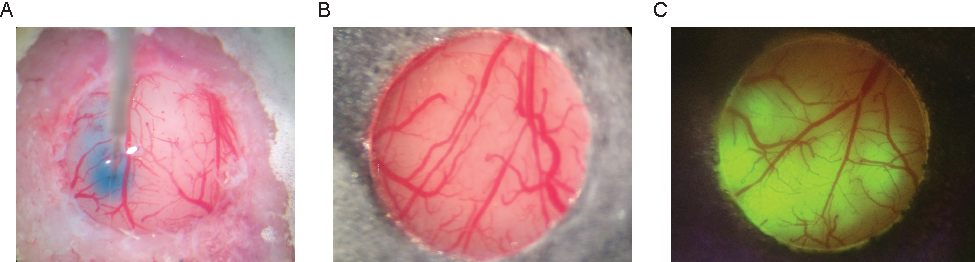
\includegraphics[width=\textwidth]{figures/chapter_2/fig_2-3_surgery_steps/fig_2-3_surgery_steps.pdf}
    \vspace{.1in}
    \caption[Chronic cranial window]{Implant of chronic cranial windows for GCaMP imaging. \textbf{A.} Exposed cortical surface and craniotomy during a microinjection of AAV-GCaMP. Blue, dye used to visualize spread (see Methods) \textbf{B.} Bright-field view of a cranial window. \textbf{C.} Fluorescent view of GCaMP expression in a cranial window.
    \label{fig:surgery_steps}}
\end{figure}

There were several possible points of attrition before a rat became viable for imaging. In our hands, viral expression was best starting at ~4 weeks post-injection. We tried various combinations of surgical steps to optimize this time-window --- for example, starting with large viral injections through a burr hole near the site of the cranial window, then waiting four weeks before exposing the cortical surface with a craniotomy-durotomy procedure and placing the coverslip window. However, for long-term window viability and high-quality imaging, we found the most reliable approach was to combine the implant surgery and the cranial window with viral injections as close in time as possible, preferably in the same surgery. When splitting the surgical steps, waiting too long (\textit{i.e.}, a week or more) compromised the structure of the skull bone, making window placement unstable and window "clouding" (growth of tissue or an inflammatory response within the cranial window that precludes imaging) much more likely. 

% Headplate assembly
In order to access lateral visual areas while keeping the rat’s head and body in a relatively natural resting position, our approach was to tilt the imaging plane relative to the animal’s head. This meant implanting the headplate at an angle that matched that of the objective. 

% Figure: Headplate and holding the rat
\begin{figure}
    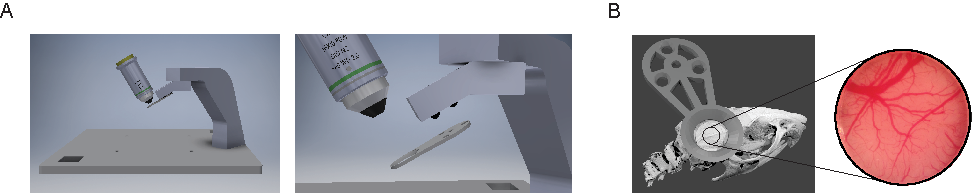
\includegraphics[width=\textwidth]{figures/chapter_2/fig_2-4_headplate_schematic/fig_2-4_headplate_schematic.pdf}
    \vspace{.1in}
    \caption[Headplate design and assembly]{Headplate design and assembly. \textbf{A.} Schematic showing the assembly for head-fixing the animal. A thick, custom-cut steel post is affixed to the platform (modular design for both habituation setups and imaging setups). An angled bracket, custom-cut to match the desired angle of the objective, contains 3 grooves that hold spherical ceramic balls (close-up, \textit{right}), which mate with the titanium headplate. \textbf{B.} Schematic of a rat skull with a custom titanium headplate positioned over the approximate location targeted for lateral extrastriate areas in the rat. Circle and inset indicate the position of the optical window implanted over these areas. A photograph of the cortical surface accessible for imaging beneath the 5-mm diameter optical window is shown to the right for illustration. 
    \label{fig:headplate_schematic}}
\end{figure}

We leveraged the high precision afforded by kinematic mounts to design custom titanium headplates that could be mounted at steep angles while preserving the capacity for precise re-positioning (Figure\ref{fig:headplate_schematic}). The headplates contained three semi-spherical grooves that mated with stainless steel ball bearings mounted to an aluminum post on the imaging platform. The headplate mated with a steel post designed to be strong enough to hold the animal stably, while keeping the view to the stimulus monitor unobstructed on one side of the animal, and on the contralateral side, sufficiently clear for the objective. Implanted animals were stably positioned at the farthest angles tested (40-45 degrees, where 0 degrees is parallel to ground, or flat on the skull).  

% %%%%%%%%%%%%%%%%%%%%%%%%%%%%%%%%%%%%%%%%%%%%%%%%%%%%%%%%%%%%%%%%
% Identifing visual areas
% %%%%%%%%%%%%%%%%%%%%%%%%%%%%%%%%%%%%%%%%%%%%%%%%%%%%%%%%%%%%%%%%
\section{Functional identification of visual areas}
% Figure: WF retino_mapping/area segmentation
Visual areas are retinotopically arranged --- each area contains a representation of the visual field called a retinotopic map, where nearby positions in physical space are represented by nearby cells on the retina, and this spatial arrangement is preserved from one part of the visual system to the next\cite{REFREF}. Conveniently, nearby visual areas have predictable ``reflections'' of retinotopic space at area boundaries. As such, distinct visual areas can be functionally identified by these mirror reflections in the representation of the visual field. To date, though several methods have been used to image neural activity in rat cortex, from intrinsic signal\cite{Gias2004} to single-photon \cite{Scott2018ImagingMacroscope} and two-photon \cite{Ohki2005, Greenberg2008} imaging, the primary visual cortex, or V1, is the only area of visual cortex to be imaged in rats.

% WIDEFIELD --------------------------------------
\subsection{A tandem-lens macroscope for wide-field imaging}
Our first step was to optically map extrastriate areas of rat visual cortex for the first time. We needed a large field-of-view (FOV) that could capture the full extent of the window (4-5$mm$ diameter). In order to ensure robust mapping with high signal-to-noise, we also needed a sufficiently shallow depth of field for avoiding out-of-focus artefacts (\textit{i.e.}, good axial resolution). To meet these needs, we developed a tilting tandem-lens epifluorescence macroscope\cite{Ratzlaff1991} (Figure\ref{fig:retino_mapping}). 

The macroscope combined two lenses in reverse configuration with a CCD camera, all custom-mounted on a rotating plate with a translating stage --- this allowed us to both rotate the imaging plane about the animal, and gave us manual control for precise positioning with manual micromanipulators. At the start of each session, we captured a high-resolution (656x492, $9.9um$ pixels) image of the surface vasculature beneath the optical window for coregistering two-photon imaging FOVs within the extents of the window. For functional imaging, we focused below the surface to ~$500um$ using micromanipulators.

% Figure:  retino_mapping (WF)
\begin{figure}
    \includegraphics[width=\textwidth]{figures/chapter_2/fig_2-5_retino_mapping/fig_2-5_retino_mapping.pdf}
    \vspace{.1in}
    \caption[Wide-field mapping]{Identifying visual area boundaries. \textbf{A.} Schematic of the tandem-lens macroscope setup used for fast mapping of the entire cranial window. \textbf{B.} Widefield, epifluorescence image of the cranial window. Scale bar, 1mm. \textbf{C.} Pseudo-colored image from phase-encoded mapping of retinotopic preference along azimuth (left) and elevation (right). \textbf{D.} Sign map calculate from the gradient of the images in \textbf{C}. \textbf{E.} Normalized power for azimuth (left) and elevation (right) mapping conditions used to threshold area maps. 
    \label{fig:retino_mapping}}
\end{figure}

\subsection{Wide-field functional mapping}
For fast acquisition of retinotopic maps, we used Fourier-based calcium imaging\cite{Kalatsky2003} (Figure\ref{fig:retino_mapping}). This approach is less time-consuming (<10 minutes) than traditional event-based paradigms in which discrete positions on a monitor are stimulated one-by-one across repeated presentations to average over noisy responses, which can take many minutes or longer. In a standard Fourier-based mapping experiment, a moving bar cycles across the screen several times at at particular frequency. The position on the screen to which a given pixel best responds corresponds to a particular part of the bar's cycle, \textit{i.e.}, the phase of response at the stimulation frequency, while how strongly a pixel responds is given by the magnitude of its response at that frequency. Calculate the phase and magnitude of response for each pixel generates a 2D map of phase and magnitude. The phase map is the retinotopic map, which we use to delineate area borders base on the mirror reflections (see Figure\ref{fig:retino_mapping}), and the magnitude map can be used to filter out unresponsive pixels (and thus, remove phase values that are meaningless). 

Visual stimuli were presented using custom Python scripts (see Methods) on a large LCD monitor, which was centered in front of the left eye to span the animal's visual field left visual field (~177$^{\circ}$ of visual angle along azimuth, 67$^{\circ}$ along elevation). The mapping protocol consisted of a periodic, moving bar stimulus\cite{Kalatsky2003, Marshel2011} presented to the (left) eye contralateral to the cranial window. The bar was either a white bar drifting over a black background or an apertured bar containing a random subset of natural scene images drifting over a gray background. We did not find an clear difference between the two bar types, but qualitatively, the latter seemed quite reliable, so we primarily used the natural scene bars for the mapping sessions. The bar was presented at 0.13 Hz along the azimuth and elevation axes, for a total of 2 (downward, rightward) or 4 (downward, rightward, leftward, upward) conditions. A total of 4-5 repetitions of 10 cycles each were acquired for each direction. 

Though we tried both intrinsic imaging and calcium imaging, we found that calcium imaging in lightly anesthetized animals was the most reliable for quickly identifying the boundaries of each visual area within a given cranial window. This precluded the need for motion correction and multiple repeated session due to animal movement, as mapping was typically done prior to habituation (see Chapter REFREF, Figure\ref{fig:experiment_workflow}). Specifically, we found that with light levels of anesthesia (minimal isofluorane, 0.5-1\%, and a small dose of choloprothixene, $2mg/kg$ REFREF), such that animals woke up immediately after the isofluorane nose cone was removed, we were able to acquire strong neural signal without needing motion correction for processing the maps.

We observed smooth retinotopic maps in  V1, LM, and LI, as well as in surrounding areas, such as AL and RL across rats (Figure\ref{fig:retino_mapping}). In some animals, the cranial window spanned all three areas, but in most cases, only one or two areas were accessible with sufficient GCaMP expression for population imaging at cellular resolution (V1: REFREF rats across REFREF imaging sites, LM: REFREF rats across REFREF imaging sites, Li: REFREF rats across REFREF imaging sites, see Methods).

% Area segmentation
To segment the visual areas, we used an established method that converts the phase map into a sign map based on the gradient of the image to determine the direction reversals, which are the area boundaries\cite{Garrett2014, Zhuang2017}. We excluded any animals that had ambiguous maps (see REFREF\ref{fig:REFREF} for examples of clear and ambiguous maps). Across animals, there was some variability in which visual areas were contained within the cranial window and the patchiness of expression due to inconsistent viral spread or injections. Patchy expression presented a challenge to a fully automated segmentation approach, for example, by splitting visual areas that should be continuous, or assigning an area where viral expression and signal was quite poor. All maps were thus inspected by eye, and patch merging and smoothing parameters were manually adjusted based on visual sign consistency, size and orientation of a given visual area relative to surrounding areas (since all windows captured minimally 1-2 mirror reflections), and comparison with movies of the imaging session, which allowed direct visualization of the stimulus traveling on the cortical surface. 

% %%%%%%%%%%%%%%%%%%%%%%%%%%%%%%%%%%%%%%%%%%%%%%%%%%%%%%%%%%%%%%%%
% Cellular resolution access
% %%%%%%%%%%%%%%%%%%%%%%%%%%%%%%%%%%%%%%%%%%%%%%%%%%%%%%%%%%%%%%%%
% 2p setup --------------------------------------
\section{A tiltable 2-photon microscope for cellular resolution}
% fig:2p_schematic (beam path, 2p schematic, face-camera, schematic of whole thing?)
% fig:scope_examples (Imaging modes:  compare 2x, 4x, also show dual channel).
% fig:multiday_imaging

% Figure:  2p schematic
\begin{figure}[t!]
    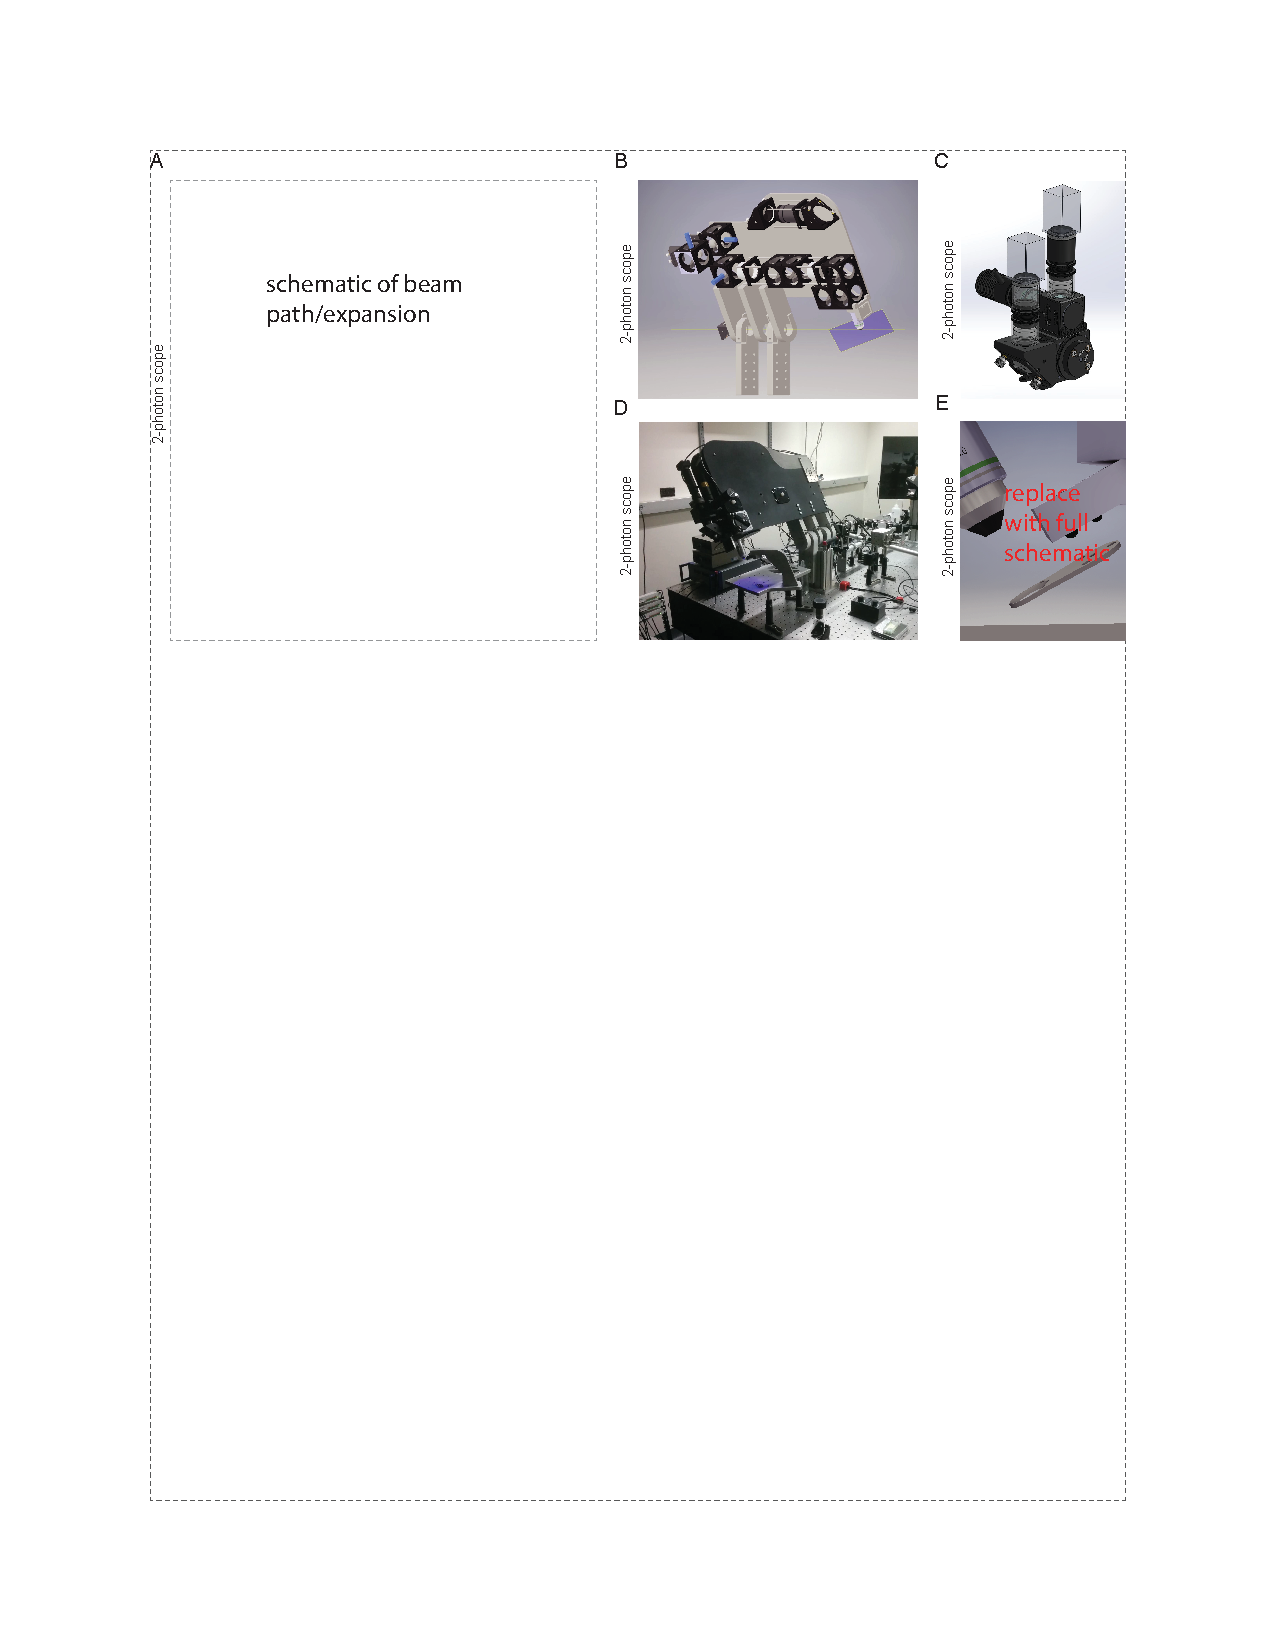
\includegraphics[width=\textwidth]{figures/chapter_2/fig_2-6_2p_schematic/2p_schematic.pdf}
    \vspace{.1in}
    \caption[Tilting two-photon microscope]{Tiltable 2-photon microscope. \textbf{A.} Schematic of optical paths to the tilting imaging plane. \testbf{B.} Schematic of the microscope housing and optical path along the rotational axis of the microscope. Optical components are included for references. \textbf{C.} An epifluorescence microscope attached to the two-photon microscope with dual-channel imaging for FOV identification one magnification step lower than the lowest two-photon zoom. \textbf{D.} A photograph of the actual microscope. \textbf{E.} A high-resolution camera system focused on one side of the animal for simultaneous imaging of face and body movements REFREF.
    \label{fig:2p_schematic}}
\end{figure}

For cellular resolution imaging, we created a custom, two-photon excitation microscope especially designed for recording from all visual areas in an awake behaving rat. A key feature of this microscope is its ability to pivot about the focal point of the microscope objective --- the microscope can be tilted to any orientation required to access lateral cortical areas while keeping the animal in a natural, unrotated position (Figure\ref{fig:2p_schematic}). Meanwhile, the body of the microscope was constructed so as to allow ample space for the animal's body while maintaining over 180º of unobstructed viewing angle for a head-fixed animal.

The microscope was built on a tilting platform that allows any region of visual cortex to be targeted, including far lateral regions. We also attached an epifluorescence imaging path for intermediate-sized FOVs (Figure\ref{fig:2p_schematic}\textbf{C}). The bright-field and epifluorescence channels are convenient for quickly identifying areas to target prior to switching into two-photon mode. On a more practical level, we were able to use the epifluorescence mode for retinotopic mapping of intermediate fields of view, in case validation with two-photon was ambiguous. 

% Pupil/face-tracking REFREF TODO.
Since we were recording neural activity in awake animals, it was critical to monitor their behavior and other facial movements, as well. Arousal states and locomotion modulate neural activity in ways that are unrelated to the task at hand or stimulus being shown to the animal. Moreover, particularly for vision experiments, the characterization of visual cortex also depends on knowing and controlling where stimuli fall on the retina. To track eye movements and all other visible behaviors that could be synced and aligned to the two-photon acquisition, we simultaneously recorded high-resolution images using an IR-illuminated camera system mounted on one side of the animal. Behavior acquisition was synced frame-by-frame to two-photon imaging acquisition with custom Python scripts for acquisition and analysis in order to track and align behavioral features, \textit{e.g.}, pupil dynamics, oral movements, etc., to all imaging data (Figure\ref{fig:2p_schematic}, TODO REFREF).

% Figure:  2p, scope_examples REFREF, 
\begin{figure}[t!]
    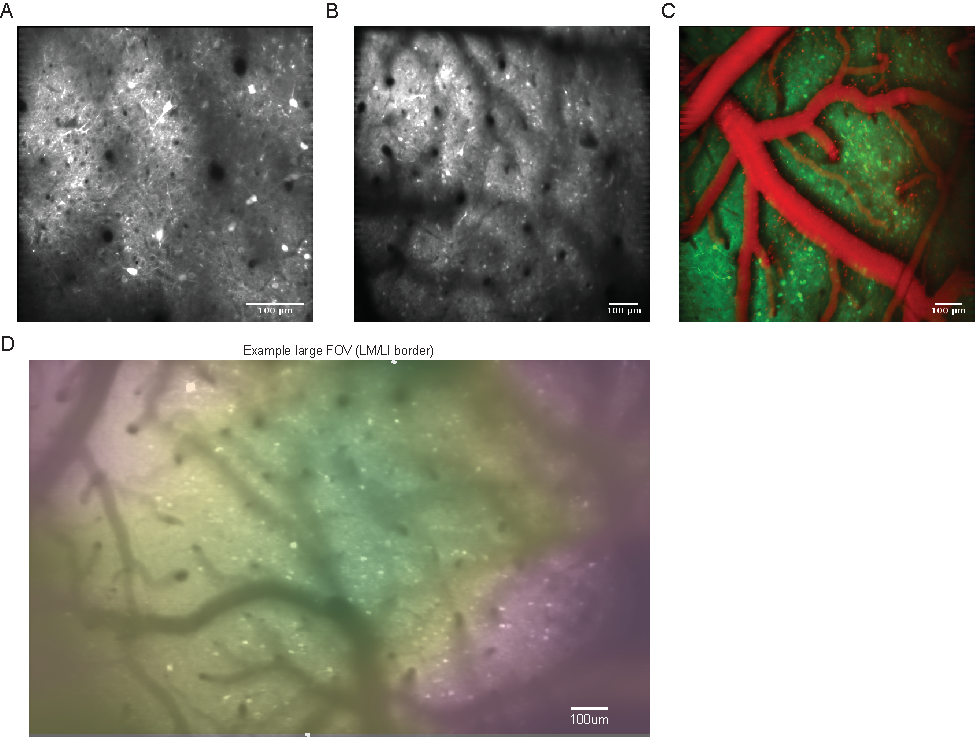
\includegraphics[width=\textwidth]{figures/chapter_2/fig_2-7_scope_examples/fig_2-7_scope_examples.pdf}
    \vspace{.1in}
    \caption[Two-photon imaging modes]{Modes of two-photon imaging. \textbf{A.} Standard FOV, $500um$ x $500um$. \textbf{B.} Standard, large FOV, $1mm$ x $1mm$. \textbf{C.} Dual-channel acqusition for red and green channels. Red, psuedo-colored SR101 blood vessel image. Green, pseudo-colored GCaMP image below the surface. \textbf{D} Extra-large FOV, $1mm$ x $1mm$, can be used for imaging two visual areas simultaneously across their border. Colormap, psuedo-colored smoothed retinotopic preferences calculated across the FOV showing the mirror reflection that demarcates the two visual areas. 
    \label{fig:scope_examples}}
\end{figure}

We created two imaging modes for the two-photon microscope (Figure\ref{fig:scope_examples}). The first is a relatively standard imaging field (up to $0.5mm$x$1mm$), with high cellular resolution (~$1um$x$1um$x$2um$ estimated point spread function, measured with a 16x/0.8NA Nikon objective). The second mode is a much larger FOV (up to $1mm$x$2mm^2$, though a standard of $1mm$x$1mm^2$ was used for most of this study, as shown in Figure\ref{fig:scope_examples}B) with slightly lower resolution (~$2um$x$2um$x$12um$ estimated point spread function). This second mode provides access to the majority of a given visual area in the rat brain, and in some cases, multiple areas simultaneously. As a proof-of-principle, we tested how well two visual areas could be identified within our largest FOV mode (~$1mm$x$2mm$). We found that a clear mirror reflection was visible when parking the objective directly above an areal boundary identified by the wide-field maps (Figure\ref{fig:scope_examples}D). In all zoom modes, the microscope supports simultaneous two-channel imaging (red and green, see Figure\ref{fig:scope_examples}C), allowing for either two functional channels (\textit{e.g.}, nuclear-localized red GECIs with green GECIs outside the nucleus), or, one anatomical channel (blood vessels filled with SR101, a fluorescent dye) for registering volumes and motion correction with the other, functional GCaMP channel. 

% Reaching our dreams 1.
% Figure:  Multi-day imaging (2 example rats)
% Figure:  2p, multiday_imaging
\begin{figure}[t!]
    \includegraphics[width=\textwidth]{figures/chapter_2/fig_2-8_multiday_imaging/fig_2-8_multiday_imaging.pdf}
    \vspace{.1in}
    \caption[Multi-day imaging]{Imaging the same cells across days. Each row shows one FOV accessed in three separate days. Each site was identified by eye. Images show the motion-corrected average for each site. No corrections to register one session with the next.    
    \label{fig:multiday_imaging}}
\end{figure}

The kinematic mount for our titanium headplate was not only designed to hold the animal stable, but importantly, to allow precise re-positioning of animals from day to day. In combination with blood vessel landmarks and the unique layout of fluorescent, GCaMP-expressing cell bodies in a given field-of-view in 3-dimensional space, this precise re-fixation allowed us to rapidly relocate the same cells across sessions (Figure\ref{fig:multiday_imaging}). It is difficult in any GCaMP-labeled brain to get the same exact population on each day, due to differences in baseline activity and generic neural tissue movement that occurs across hours. However, the majority of well-labeled cells combined with scanning in depth enabled good matching across sessions. 

% Habituation + shaping
To reduce prohibitively large motion artefacts from rats resisting head-fixation, we developed a shaping procedure to habituate rats for multi-hour sessions (the longest sessions were ~5 hours). Briefly, rats were placed in a red, transparent cylinder also used as enrichment in their home cages, and over the course of several days ($\sim$2-4 days) animals were given decreasing doses of sedative (Midazolam, REFREF mg/kg) and increasingly long habituation sessions (gradually increasing from $\sim$30 minutes to $\sim$3 hours). We found that rats always struggled in the first habituation session without any sedative, which appeared to be critical to accustom the rats to head-fixation in long sessions. That is, most rats quickly learned that it was not possible to physically remove themselves from the implant. We found even in the first two-photon imaging sessions, rats struggled at the very start, well before acquisition began, and remained quiescent throughout most of the session. Although we did not train animals on a task, observable signs indicated that the animals were relatively calm --- they groomed periodically throughout the session, and accepted water and ate treats while they were head-fixed. 

%%%%%%%%%%%%%%%%%%%%%%%
% Concluding remarks
\section{Concluding remarks}
The methodological developments presented in this chapter provide a reliable series of steps for long-term imaging of cranial windows in awake rats. Many of these methods are readily available in mice, and the past decade of systems neuroscience research has seen the surprising emergence of mice as a powerful model system for studying visual circuits. However, the rat has been an important model across all fields of biology for much longer, from sensory behavior\cite{Lashley1930, REFREF} to spatial navigation\cite{REFREF}, to physiological disorders and drug testing\cite{REFREF}. 

We overcome several challenges that have prevented the use of a subset of immensely powerful tools in rat models. First, we developed methods for stably holding an animal by its head, while leaving the rest of its body free to either sit relatively naturally or engage with manipulanda relevant for a behavior task. Second, we fine-tuned standard surgical protocols for cranial window implants that would allow long-term viability for cellular resolution imaging in awake rats. 

Importantly, we demonstrate a method for accessing some of the most lateral and posterior areas of rat cortex. The combination of hard-to-access imaging planes and the rat's capacity for producing large (and damaging) mechanical forces extremely presented significant challenges. Our custom designs for tiling imaging systems overcome these challenges by rotating the optical axis around the animal, allowing a relatively natural sitting position, which is important both for keeping the animal calm during imaging as well as comfortable enough to willingly engage in behaviors. 

We engineered a two-photon microscope design that allows a full repertoire of imaging modes, including multi-channel acquisition and large fields of view that can allow multiple areas to be imaged simultaneously in the rat. These developments unlock significant avenues of research in rats, particularly in questions involving complex behavior and the various functions of different cortical areas, and the nature of their dynamics during learning or particular behaviorally-relevant contexts. 

%%%%%%%%%%%%%%%%%%%%%%%
% While previous studies have shown used coarse retinotopy to identify the areas in which they were recording, the fine-scale retinotopic organization of cell bodies in any extrastriate area remains unknown. To characterize retinotopic preferences at single-cell resolution, we used the same phase-encoding Fourier paradigm used in wide-field mapping with two-photon calcium imaging.


% % Retino scatter
% Cell bodies exhibited a coarse-scale retinotopic organization. However, retinotopic preferences of neighboring cells were disordered and deviated from the surrounding neuropil in V1, LM and LI {\fig:Figure1f, REFREF, Supplemental 2.2, 2.3, stats REFREF}, consistent with findings in mouse visual cortex \cite{Liang2018, Andermann2011, Marques2018}. Single sweeps of the stimulus evoked robust responses in individual cells. 


% We found an asymmetric expansion of spatial representation along the elevation axis in all areas tested (Figure\ref{fig:2p_retino}). There was a ~2-fold increase in cortical magnification along the visual axis of elevation versus azimuth (REFREF paired t-test, V1: p=#, LmL p=#, Li: p=#). 
\begin{savequote}[75mm]
Nulla facilisi. In vel sem. Morbi id urna in diam dignissim feugiat. Proin molestie tortor eu velit. Aliquam erat volutpat. Nullam ultrices, diam tempus vulputate egestas, eros pede varius leo.
\qauthor{Quoteauthor Lastname}
\end{savequote}

\chapter{Basic characterizations}
% Figure:  RF mapping, examples
% Figure:  RFs, aggregate/summary plots
% Figure:  GRATINGS, stimuli + example traces
% Figure:  Summary stats of OSI, DSI, "Fraction tuned"
% Figure:  RFs + ORI preferences

\newthought{Lorem ipsum dolor sit amet}, consectetuer adipiscing elit. Morbi commodo, ipsum sed pharetra gravida, orci magna rhoncus neque, id pulvinar odio lorem non turpis. Nullam sit amet enim. Suspendisse id velit vitae ligula volutpat condimentum. Aliquam erat volutpat. Sed quis velit. Nulla facilisi. Nulla libero. Vivamus pharetra posuere sapien. Nam consectetuer. Sed aliquam, nunc eget euismod ullamcorper, lectus nunc ullamcorper orci, fermentum bibendum enim nibh eget ipsum. Donec porttitor ligula eu dolor. Maecenas vitae nulla consequat libero cursus venenatis. Nam magna enim, accumsan eu, blandit sed, blandit a, eros.



\section{Lateral visual cortex exhibits many of the same core properties found in primates}

Since we have demonstrated the key prerequisite of establishing the behavioral ability of rats to perform visual recognition has been established, we next turned our attention to the neuronal substrates of these abilities.  Primate visual cortex is arranged hierarchically, with visual inputs from the thalamus first arriving in so-called ``striate'' cortex (also known as area V1), before being processed and forwarded through a successive chain of hierarchically-organized visual areas (area V2 > area V4 > inferotemporal cortex) curving along the ventral surface of the brain.  

Several key trends have been observed in the response properties of visual neurons as one progresses from ``lower'' to ``higher'' visual areas along this ventral pathway. First, the region of visual space that a given cell responds to (the ``receptive field'') gradually increases as one moves along the ventral pathway, with receptive fields in the highest stages of visual cortex sometimes responding to up to half of the visual field \cite{op2000spatial}. Meanwhile, selectivity for complex object features also increases along the ventral visual pathway, with neurons in later stages of the pathway responding only to very particular configurations of features \cite{Desimone1984, Logothetis1996}.  Critically, as one progresses along the ventral pathway, neurons also exhibit greater tolerance to identity-preserving transformation of the retinal image -- that is, neurons tend to retain their selectivity for particular object features even if those features are, for instance, moved around on the retina, or scaled up or down in size \cite{Ito1995}.These combined features of selectivity and tolerance are in many ways the key computational hallmarks of high-level vision \cite{DiCarlo2007, DiCarlo2012}. 

Anatomical studies have shown that the connectivity of rodent visual cortex observes a similar hierarchical pattern, with thalamic inputs arriving in an analogous striate area V1 in posterior of the brain, and then projecting ventrally to a series of interconnected extrastriate areas  \cite{Coogan1993, ETC}.  However, while these areas have been characterized anatomically, very little is known about their function.


% \begin{savequote}[75mm]
% Nulla facilisi. In vel sem. Morbi id urna in diam dignissim feugiat. Proin molestie tortor eu velit. Aliquam erat volutpat. Nullam ultrices, diam tempus vulputate egestas, eros pede varius leo.
% \qauthor{Quoteauthor Lastname}
% \end{savequote}

\chapter{Object representations in lateral visual cortex}
\newthought{Shape is a diagnostic feature} of object identity. Visually similar objects, such as a pear and an apple, can be grouped together by certain shared visual features. On the other hand, different images or views of any one object can look dramatically dissimilar, yet still belong to the same object. The ventral visual pathway in the primate brain is thought to transform non-diagnostic, low-level representations of features that may be common to many different objects into high-level representations that are both diagnostic of object identity, or selective for a given object, and robust to variations in particular appearance, or tolerant to identity-preserving transformations. In the first chapter, we established the behavioral ability of rats to perform visual object recognition and quantified their perceptual choices of object similarity. We next turned our attention to the neuronal substrates of these abilities. 

% Neural subtrates of object recog. -- what do we know from primates.
Primate visual cortex is arranged hierarchically, with visual inputs from the thalamus first arriving in so-called ``striate'' cortex (also known as area V1), before being processed and forwarded through a successive chain of hierarchically-organized visual areas (area V2 > area V4 > inferotemporal cortex) curving along the ventral surface of the brain. Along each stage of the ventral stream, there is a gradual increase in object selectivity and tolerance, culminating in area IT, at the highest level of the ventral pathway. 

Several key trends have been observed in the response properties of visual neurons as one progresses from ``lower'' to ``higher'' visual areas along this ventral pathway. First, the region of visual space that a given cell responds to (the ``receptive field'') gradually increases as one moves along the ventral pathway, with receptive fields in the highest stages of visual cortex sometimes responding to up to half of the visual field\cite{OpDeBeeck2001}. Meanwhile, selectivity for complex object features also increases along the ventral visual pathway, with neurons in later stages of the pathway responding only to very particular configurations of features\cite{Desimone1984, Logothetis1996}. Critically, as one progresses along the ventral pathway, neurons also exhibit greater tolerance to identity-preserving transformation of the retinal image -- that is, neurons tend to retain their selectivity for particular object features even if those features are, for instance, moved around on the retina, or scaled up or down in size\cite{Ito1995}.These combined features of selectivity and tolerance are in many ways the key computational hallmarks of high-level vision\cite{DiCarlo2007, DiCarlo2012}. 

% Previous rodent studies
% \section{Lateral visual cortex exhibits some of the same core properties found in primates}
Anatomical studies have shown that the connectivity of rodent visual cortex observes a similar hierarchical pattern, with thalamic inputs arriving in an analogous striate area V1 in posterior of the brain, and then projecting ventrally to a series of interconnected extrastriate areas\cite{Coogan1993}. However, while these areas have been characterized anatomically, much less is known about their function. Most of what we know about rat visual cortex beyond V1 comes from single-unit, electrophysiology studies that have characterized response properties of neurons in the context of visual object recognition\cite{Tafazoli2017, Vermaercke2014, Vinken2014}. While these studies differ in a few points (see Conclusion), a few key trends have been observed. First, all studies to date report an increases in receptive field size from V1 to LM to LI and beyond\cite{Tafazoli2017}. This is consistent with studies of extrastriate cortex in mice\cite{Murgas2020, Siegle2021}, as well as my characterizations from the previous chapter. Second, though there is not yet a clear consensus, several studies report increased shape selectivity or shape discriminability for single-units in extrastriate cortex\cite{Tafazoli2017, Vermaercke2014, Vermaercke2015, Vinken2016}. Finally, most studies report some degree of tolerance to identity-preserving transformations: single-units recorded in extrastriate cortex along these lateral areas maintain shape selectivity or discriminability across changes in position, size, or rotation\cite{Vermaercke2014, Tafazoli2017}.

At the same time, mouse visual cortex has been characterized to an unprecedented degree, such that arguably more is known about the mouse visual system that that of any primate (see \cite{Niell2021} for a review). These studies present a growing body of discoveries that indicate that, despite many apparent similarities between rodent and primate visual system, there may be many ways in which the two are signficiantly different. For example, several studies have found asymmetries in visual field representations and direction tuning preferences in mouse visual cortex\cite{Zhuang2017, Liang2018, Sit2020, Murgas2020}. In addition, the deep, hierarchical organization evident in primate visual cortex seems to be quite different in rodent visual cortex. For example, area POR, a higher-order visual area in the mouse, receives most visual input via the superior colliculus (SC), and not V1 by way of the dLGN\cite{Beltramo2019a}. This means that unlike in primates, where V1 is the gateway for visual information through the ventral path, mice have a separate pathway to higher-orer visual areas --- silencing V1 activity does not affect motion-processing activity of POR cells. Thus, in the context of visually-driven behavior, such as motion perception or, in this case, visual object recognition, rodent and primate visual systems may have different principles of organizations or species-specific solutions for a given behaviorial need. 

To determine the extent to which rat lateral visual cortex intrinsically exhibits properties thought to be important for spontaneous, as opposed to learned, object recognition behavior, I recorded from neural populations in awake, naive rats presented with a subset of the same stimuli tested on the trained rats (see Chapter 1, Figure\ref{fig:behavior_generalization}). The goal of these experiments was to investigate how neural responses reflect changes in shape that are due to transformations along identity-changing axes or transformations along identity-preserving axes.

% ---------------------------------------------------------------
% Single neuron selectivity and tolerance
% ---------------------------------------------------------------
\section{Single neurons exhibit selectivity and tolerance}
\begin{figure}[t!]
    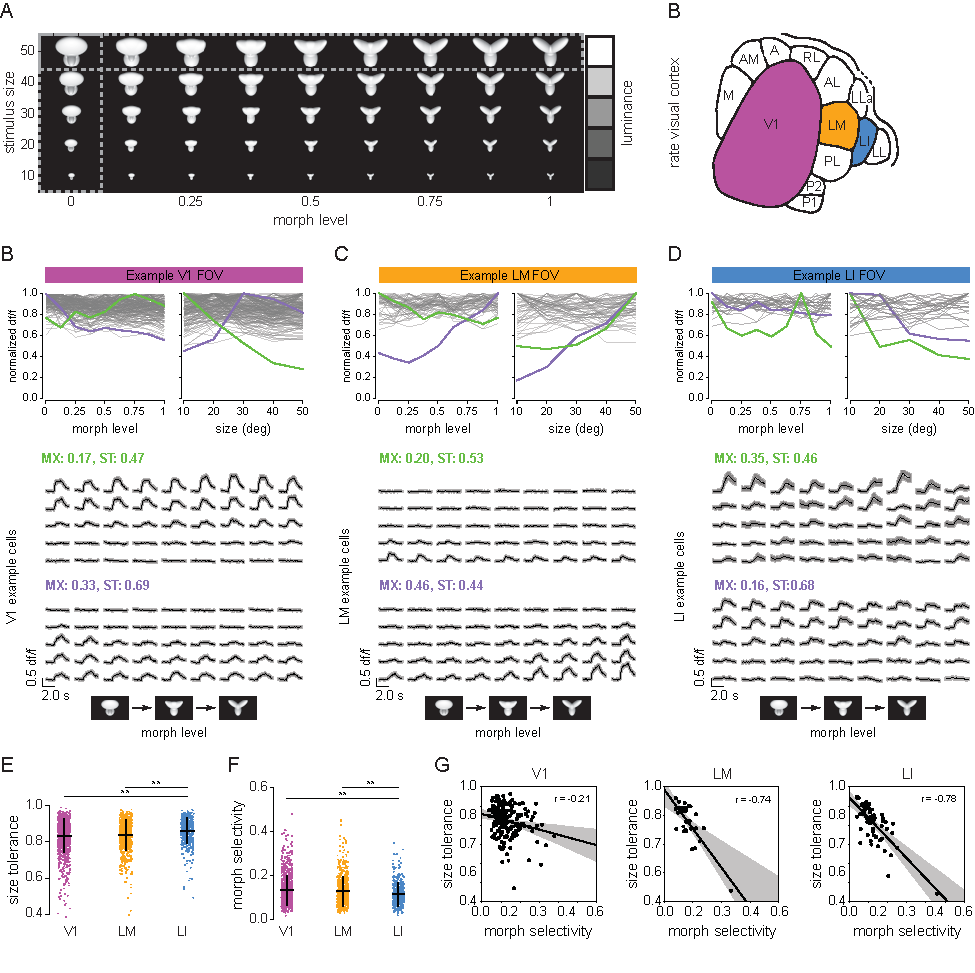
\includegraphics[width=\textwidth]{figures/chapter_4/fig_4-1_single_cell_selectivity_tolerance/fig_4-1_single_cell_selectivity_tolerance.pdf}
    \caption[Single neuron selectivity and tolerance]{Selectivity and tolerance. 
    \textbf{A.} Transformations tested: 5 stimulus sizes (identity-preserving) and 9 morph levels (identity-changing). 5 luminance stimuli (fullscreen) were matched for each size
    \textbf{B.} Rat visual areas in this study. 
    \textbf{C.} Morph selectivity (left) and size tolerance (right) for an example V1 FOV. Black lines, single cell tuning profiles. Color lines, example cells: Green, the first set of traces (middle). Purple, the lower set (bottom). Time courses arranged as in \textbf{A}. Lines and shading, mean and SEM across repeats.
    \textbf{D.} Same as \textbf{C}, but for an LM FOV.
    \textbf{E.} Same as \textbf{B} and \textbf{C}, but for an LI FOV.
    \textbf{F.} Distributions of size tolerance for V1, LM, and LI cells. Each dot is a cell, black lines denote mean and SD across cells.
    \textbf{G.} Same as \textbf{F}, but for morph selectivity. 
    \textbf{H.} Correlation between size tolerance and morph selectivity for example V1 (left), LM (middle), and LI (right) FOVs. Each dot is a cell. Line and shading, linear fit and 95\% CI.
    \label{fig:selectivity_tolerance}}
\end{figure}

One key feature of the primate ventral stream is a gradual increase in shape or object selectivity and a parallel increase in tolerance to identity-preserving transformations. Previous studies have shown that single-units in area IT of monkeys exhibit a trade-off between these properties: neurons that are highly selective are less tolerant to identity-preserving transformations and highly tolerant neurons are not as selective to particular objects\cite{Zoccolan2007}.

To determine whether single neurons exhibited similar characteristics in rat visual areas, I first measured single neuron response profiles in areas V1, LM, and LI. For identity-changing transformations, I tested a subset of the morphs used to test the naive perceptual boundaries between the anchor objects in trained animals (Figure\ref{fig:selectivity_tolerance}A). For identity-preserving transformations, I tested a subset of sizes covering the range of stimulus sizes used to test behavioral generalization performance (see Chapter 1, Figure\ref{fig:behavior_generalization}). Since size changes come with large changes in luminance, I also presented a subset of full-screen stimuli that were assigned luminance-matched grayscale values for each size tested (see Methods).

All areas contained a diverse range of object selective and size tolerant cells. For example, some cells exhibited size tuning but did not differentially repsond to the different morphs, while other cells exhibited tuning to particular morphs, without showing response modualtion to the different sizes. Still others appeared to be tuned to overall luminance, showing selective responses to the fullscreen stimuli and no responses to shapes. Overall, I found that across the tested object stimuli, cells in LI had the lowest lifetime sparseness, while cells in V1 and LM were similarly high in sparseness (Mann-Whitney U-test, p<0.01, corrected for mulitple comparisons with the Benjamini/Hochberg method). Since changes in object shape were due to both variation in morph level and in stiulus size, the sparseness observed in V1 and LM could reflect a higher selectivity for morph shapes or a lower tolerance to varying size. To quantify the amount of object selectivity and tolerance, I calculated a morph selectivity index (MX) and a size tolerance index (ST) for each cell\cite{Zoccolan2007}. I found a range of tuning profiles across cells that was comparable between the three areas (Figure\ref{fig:selectivity_tolerance}B-D). On average, LI cells were both less selective to morph shape and more tolerant to changes in size, relative to cells in V1 and LM (Figure\ref{fig:selectivity_tolerance}E-F). Notably, this difference was not attributable to overall lower response magnitudes in LI: although there were relatively fewer LI cells responsive to the object stimuli overall, of the cells that were responsive, response magnitudes were comparable across areas (see Table\ref{tab:data_counts}).

It is possible that the relatively higher average morph selectivity in V1 and LM cells reflects greater sensitivity to overall luminance values. To characterize the extent to which size or morph tuning simply tracks luminance sensitivity, I compared tuning for size to tuning for the fullscreen luminance stimuli. Specifically, I calculated the correlation between each cell's tuning curve for all sizes for its preferred morph object, and its tuning curve for the size-matched luminance stimuli. While there were indeed cells whose size- or morph-tuning profiles were tightly correlated with broad luminance levels, this was not the case for the majority of cells (V1: 9.8+/-6.8\% of cells with significant correlation between size and luminance tuning; LM: 12.6+/-8.2\%; Li: 12.2+/-9.1\%, see Figure\ref{supfig:luminance_corr}). 

To determine whether single neurons in rat visual cortex exhibit a similar trade-off between shape selectivity and transformation tolerance as observed in primate IT, I calculated the correlation between morph selectivity and size tolerance for simultaneously recorded cells in each imaging site (Figure\ref{fig:selectivity_tolerance}H). I found a strong, negative correlation between morph selectivity and size tolerance for areas LM and LI. Notably, these features were also negatively correlated in V1 imaging sites, but to a weaker degree. To determine whether the strength of this trade-off differed between the three areas, I performed a shuffle test in which I scrambled each cell’s selectivity index and tolerance index, then recalculated the tradeoff metric (correlation coefficients). When comparing populations that passed this shuffle test (p<0.05 over 5000 iterations), I found that correlation coefficients for LM and LI populations were significantly more negative than those in area V1 (Mann-Whitney U test, p<0.05 Bonferroni-corrected for multiple comparisons), suggesting that on average, the negative relationship between selectivity and tolerance was stronger for LM and LI FOVs.

% A critical property of single neurons in IT is the preservation of rank-ordered object selectivity, that is, relative tuning preference for a set of objects is maintained across changes in identity-preserving transformations such as position or size\cite{Li2009, REFREF}. 

% ---------------------------------------------------------------
% Arousal
% ---------------------------------------------------------------
\section{Arousal modulates tuning properties} 
\begin{figure}[t!]
    \includegraphics[width=\textwidth]{figures/chapter_4/fig_4-2_arousal/fig_4-2_arousal.pdf}
    %\vspace{.1in}
    \caption[Arousal modulates tuning]{Arousal modulates tuning. 
    \textbf{A.} Example view of the face-tracking camera pointed at the animal’s face, overlaid with face feature annotations for whiskers and pupil tracking.
    \textbf{B.} Example pupil diameter trace (top) and neural responses (bottom) for repeated presentations of a single condition type. Gray bars in the middle show the stimulus period of each trial. Colormap shows z-scored responses.
    \textbf{C.} Response magnitude on trials in which animals were in “high” (magenta) and “low” (cyan) arousal states (i.e. trials with an average pupil diameter above or below the 67th and 33rd percentiles, respectively). Points, average response magnitude across cells of a given imaging site. Error bars, SD.
    \textbf{D.} Size tolerance as a function of arousal state, for each visual area. Points, average response magnitude across cells of a given imaging site. Horizontal bars, average across sites for a given visual area. Error bars, SD.
    \textbf{E.} Morph selectivity as a function of arousal state, for each visual area. Notation as in \textbf{E}.
    \textbf{F.} Correlation coefficient for morph selectivity versus size tolerance as a function of arousal state, for each visual area. Notation as in \textbf{E}, \textbf{F}.
    \label{fig:arousal}}
\end{figure}

Tuning preferences are known to be modulated by the behaviorial state of the animal, such as overall arousal or locomotion\cite{Niell2010,Saleem2013,Vinck2015, Dadarlat2017}. Even in the absence of visual stimulation, neural activity in visual cortex can be driven and modulated by locomotion or facial movements\cite{Keller2012SensorimotorMouse, Stringer2019a}. A key advantage of recording in head-fixed rats was the ability to simultaneously monitor facial movements of the animals with (Figure\ref{fig:arousal}A-B). Face video was acquired simultaneously and synced with neural acquisition (see Methods). From these data, a rich repertoire of facial and front-of-body movements could be extracted for every frame, including eye position, pupil size, whisker positions, snouth and mouth locations, as well as paw positions. These features were extracted\cite{Mathis2018, Nath2019} and aligned to neural activity, as I designed the acquisition pipeline to sync with that of the neural acquisition pipeline (see Supplementary Information).

% pupil 
Decades of research in pupillometry in humans, nonhuman primates, and rodents support the view that changes in pupil diameter track not only changes in luminance, but also changes in alertness, attention, and effort, or broadly, levels of arousal\cite{Reimer2016, McGinley2015WakingResponses, Reimer2014, Vinck2015}. Arousal states, as measured by methods from pupillometry, have been shown to modulate both single neuron tuning and population decodability. To characterize how broad changes in arousal modulate the visual response properties of cells tuned to the object stimuli, I compared neural activity between high and low arousal states, as measured by changes in pupil size\cite{Liang2020, Stringer2019a}. Specifically, trials were separated into ``high'' or ``low'' states based on pupil size. Since pupil diameter changes with luminance changes, as well, care was taken to sample the range of pupil sizes within each stimulus condition (see Methods). 

I compared single cell measures of size tolerance and shape selectivity, as well as linear separability of population representations across areas V1, LM and LI. Consistent with previous studies of arousal modulation in V1, I found that response magnitudes were greater when the animal was in a high arousal state, as compared to a low arousal state, and this was also true for areas LM and LI (Figure\ref{fig:arousal}C). Across these visual areas, shape selectivity was also greater, and size tolerance lower, in high arousal states (Figure\ref{fig:arousal}D-E). That is, increased arousal was correlated with overall increases in selectivity.

To see whether the previously observed trade-off between selectivity and tolerace was modulated by arousal, I also quantified the correlation between the two for high and low arousal states. Interestingly, in V1, but not in LM and LI, the strength of this relationship, as measured by the size of the correlation coefficient between tolerance and selectivity, was weaker in high arousal states (Figure\ref{fig:arousal}F). The reduced strength of the negative correlation between selectivity and tolerance may be predictable if, on average, increases in morph selectivity result in increases in size tolerance (\textit{i.e.}, a less steep slope for the correlation plots shown in Figure\ref{fig:selectivity_tolerance}H). However, that this is not evident in LM and LI populations, despite all three areas exhibiting similar increases in selectivity for high arousal states, suggest that these populations are relatively more robust to arousal differences at the level of individual cells. 


% ---------------------------------------------------------------
% Morphs
% ---------------------------------------------------------------
\section{Single cells show object discriminability}
% Morphs -- neurometric curves, single-neuron disriminability
% 
Overall, though I observed a slight increase in size toleranace and a slighty decrease in morph selectivity comparing across areas V1 to LM to LI, the distributions of selectivity and tolerance metrics were broad and otherwise quite similar for all there areas. One concern with the observation that the greater size tolerance in LI could be due to LI cells simply not having any preference at all for the particuar shapes being presented, despite being visually responsive.  
I previously showed that trained rats are capable of discriminating between object A and object B, and that their determination of the morph shapes varied as a function of how similar a given morph shape was to either A or B (see Figure\ref{fig:behavior_generalization}). However, in the naive rats, there was no reason for cells to prefer one object over the other. Nonetheless, it was possible to quantify the extent to which a given cell intrinsically, or at least, without training or experience, demonstrates strong selectivity for one or the other shapes, based on its ability to discriminate between the stimuli.

For an ideal observer discriminating between object A and object B based on neural activity, the distributions of responses to A and responses to B would be perfectably separable. Similar to the way behaving rats were trained to discriminate A and B, I first selected a subset of cells that did exhibit selectivity to one anchor over the other (see Methods), and then used a receiver-operating-characteristic (ROC) analysis from signal detection theory to determine how well a cell could discriminate its preferred object from the other morphs\cite{Green1966, Britten1992, Busse2011}. In other words, neural performance was based on the capacity of an ideal observer to discriminate whether A or B was shown based on each neuron's distribution of responses:  this analysis assumes that the cell has a ``decision boundary'' where anything falling to the right (larger responses) is the preferred object, and anything falling below (smaller responses) is the non-preferred, or null, object. Based on the cell's response distributions for object A and object B, I calculated an ROC curve, where each point depicts the fraction of trials on which the preferred object exceeded criterion level, plotted against the proportion of trials on which the null object response exceeded criterion. When discrimination is high, the area under the ROC curve (AUC) is closer to 1; when discrimination is at chance, AUC is close to 50\%. 

\begin{figure}[t!]
    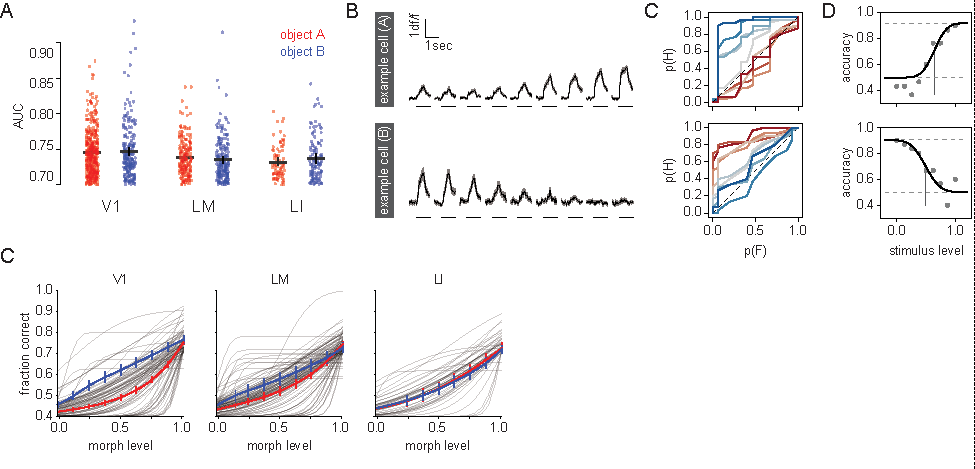
\includegraphics[width=\textwidth]{figures/chapter_4/fig_4-3_neurometric/fig_4-3_neurometric.pdf}
    %\vspace{.1in}
    \caption[Single neuron discriminability]{Single neuron discriminability. 
    \textbf{A.} Distribution of discriminability (AUC) for cells selective for either object A (red) or object B (blue), which were the two anchor objects.
    \textbf{B.} \textit{Top}, Example time courses at each morph level at the preferred size for a cell preferring object B. \textit{Bottom}, Example time courses for a cell preferring object A. Horizontal bar, stimulus period. 
    \textbf{C.} \textit{Top}: Example ROC curves for the cell shown in \textbf{B}, \textit{top}. The area under these curves (AUC) measures how well a neuron discriminates one image, the preferred object B, from each other image, or the other morph levels. Red corresponds to object A (morph level 0\%B) and blue corresponds to object B (morph level 100\%B). \textit{Bottom}: ROC curves, but for the cell shown in \textbf{B}, \textit{bottom}. 
    \textbf{D.} \textit{Top}: Corresponding neurometric curves fit to the AUC values at each morph level for the cell shown in the top panels of \textbf{B} and \textbf{C}. \textit{Bottom}: Corresponding neurometric cures for the cell shown in the bottom panels of \textbf{B} and \textbf{C}. 
    \textbf{E.} Neurometric curves for all selective, well-fit cells in V1 (left), LM (middle), and LI (right). Only cells that passed criterion performance (70\% accuracy) were tested on the intermediate morphs, then fit for their ability to discriminate the objects as a function of morph level. Thin gray lines correspond to individual cells. Red, mean and SD across cells preferring object A. Blue, mean and SD across cells preferring object B.
    \label{fig:neurometric}}
\end{figure}

In contrast to the concern that high size tolerance simply reflected low shape selectivity, I found that selective cells in all visual areas exhibited strong discrimination capacity for the anchor objects Figure\ref{fig:neurometric}A). While LI had fewer cells that were selective, as previously noted, of the cells that were selective, there was no apparent difference in single neuron discriminability across the visual areas. 

When testing the behaving animals, rats first had to pass a criterion performance level of at least 70\% accuracy --- only rats that demonstrated clear discrimination performance were included in tests of perceptual similarity along the morph continuum. However, since the rats imaged here were not trained, the anchor objects did not have any particular meaning: it was not necessarily the case that cells should faithfully track the shape continuum from one anchor extreme to the other. Rather, a cell could selectively prefer one of the intermediate morphs (for example, the green cell shown under LI in Figure\ref{fig:selectivity_tolerance}E). In order to determine the extent to which neural responses reflected the physical transformations along the morph axis, I calculated corresponding neurometric curves for cells selective to one or the other anchor. For cells preferring object A (or morph level 0\%B), ROC curves were calculated to determined how well the cell could discriminate each morph from its non-preferred object B (or morph level 100\%B), and vive versa for cells preferring object B (Figure\ref{fig:neurometric}C). As before, I then calculated the AUCs, not just for the extreme anchors, but for the intermediate morphs, and quantified how the AUC values varied as a function of morph level to create neurometric curves (Figure\ref{fig:neurometric}D). In all cells with neurometric fits, most were biased toward the stimulus level of maximum difference between the two objects (Figure\ref{fig:neurometric}E). This was expected to some degree, as only cells that were successful at discriminating objects and selective for one anchor over the other were included. 

Interestingly, although average neurometric curves were similar for cells in LM and LI, this was not the case for V1 cell, as cells preferring object A tended to be more biased than cells preferring object B: the average curve for B-preferring cells was relatively well-centered, while the curve for A-preferring cells were biased toward the side of the preferred object (Figure\ref{fig:neurometric}E). In addition, there were more B-preferring cells than A-preferring cells in V1. Compared to object A, object B has qualitatively more linear or elongated features (see Figure\ref{fig:basic_training}A). As such, it is possible that the reduced bias in the neurometric curve for B-selective cells is a result of more even representation by cells with strong perferences for the edges defining the morph space between the two objects.

% REFREF, jnd, compare with behavior? 

% ---------------------------------------------------------------
% Population responses
% ---------------------------------------------------------------
\section{Population responses are linearly separable}
Notably, the trained rats have access to much more than a single neuron during the behavior task. Thus, I next asked how the obejct stimuli are represented at the level of neural populations. How the brain achieves the critical combination of high object selectivity with high tolerance to particular views remains a mystery. As observed in primate IT, single-units exhibit these properties as a trade-off, where one comes at the cost of the other\cite{Zoccolan2007}. I found a similar observation at the single cell level, but notably, the tradeoff was relatively comparable across areas, albeit with a weaker relationship in V1 (Figure\ref{fig:selectivity_tolerance}H). In primates, it is thought that each successive stage of the ventral stream computes a series of operations that make object representations increasingly linearly separable. Since trained rats accurately classified novel image transformations in the absence of any feedback, this suggested that explicit training was not required for generalization behavior (see Figure\ref{fig:behavior_generalization}). I thus asked whether neural populations in naive rats exhibit signatures of these ventral-stream-like computations thought to be important for tolerant visual object representations.

\begin{figure}[t!]
    \includegraphics[width=0.9\textwidth]{figures/chapter_4/fig_4-4_neural_generalization/fig_4-4_neural_generalization.pdf}
    %\vspace{.1in}
    \centering
    \caption[Population representations of objects]{Linear separability and tolerance. 
    \textbf{A.} Schematic of discriminability for neural populations. A hypothetical population response for 1 presentation of an image as a point in N-dimensional space (example shows a population of size N=2 for illustration). Different trials of the same image (red) form a cloud in this N-D space, while trials of a different image (blue) form another cloud (left). The ability of the population to discriminate the images is proportional to how far apart the response clouds are. Linear classifier approaches identify the optimal hyperplane that separates one image (red) from the other (blue). Performance is measured as the proportion of times that response vectors fall on the correct side of the hyperplane (right). 
    \textbf{B.} \textit{Left}: A population that supports generalization under one test (dashed line) but fails under another (solid line) for different, novel views (red, open circles) of an object. \textit{Right}: A population that passes tests of generalization when testing on a single training condition (solid line in \textit{left}), as illustrated by the response vectors for both novel and trained views falling on the correct side of the hyperplane.
    \textbf{C.} Linear separability as a function of population size (see \textbf{B}, left) for V1, LM, and LI. Classifiers were trained on with responses from all sizes. Dotted, shuffled labels. Error bars, bootstrapped estimates of the 95\% CI of the mean accuracy. 
    \textbf{D.} Generalization test accuracy (see \textbf{B}, right) by population size for V1 (left), LM (middle), and LI (right). Classifiers were trained at 1 stimulus size, then tested on new samples of the same (black) or novel stimulus sizes (blue). Dotted lines and error bars as in \textbf{C}.
    \textbf{D.} Generalization score (ratio of novel to trained) split by the difference between train and test stimulus sizes (N=128 cells).
    \textbf{E.} Generalization test accuracy at each trained stimulus size. Classifiers were trained with 4 out of 5 stimulus sizes, then tested on different trials of the training size (black) or on new trials of the held-out, novel size (blue), for all combinations of train/test sizes. Error bars, SD across imaging sites. Dotted lines, shuffled labels.
    \label{fig:neural_generalization}}
\end{figure}


However, during behavior, the animal has access to much more than the activity of a single neuron. To determine the extent to which neural populations in rat visual cortex are inherently capable of representations that support discrimination and generalization, we took a population-based approach to compare areas V1, LM, and LI in awake, but untrained rats. Specifically, we trained linear SVMs with neural responses to these same object images to classify the responses as belonging to object A or object B \cite{Hung2005, Li2009, Rust2010SelectivityIT}. We then tested the classifiers on each of the two types of generalization tasks performed by the trained rats. 

Before testing the ability of each population to generalize across identity-preserving transformations, we first tested how well the objects could be discriminated from each other at each of the tested transformations. That is, if a given population failed to discriminate the objects at a given size, failure to generalize to that size would be trivial. For each imaging site, or set of simultaneously recorded cells, in each visual area, we trained linear classifiers to discriminate the two objects at each size, then scored accuracy on trials of the same condition that the classifier had never seen. To avoid trivial generalization due to poor baseline performance, only those populations with average test accuracies greater than accuracies calculated from shuffled object labels were included. 

To test discriminability of the two anchor objects, we first tested neural representations under a ``Train 1, test same'' regime: At each stimulus size tested, we trained classifiers to discriminate object A from object B. Overall, discrimination accuracy improved with increasingly larger stimulus sizes. This is consistent with previous single-unit studies of aggregated populations, though here we report performance for simultaneously recorded populations. This stimulus size dependence was present in all visual areas, and notably, overall performance was comparable across areas, as well. Specifically, average test scores were similar for populations in V1, LM, and LI, with mean scores in V1 and LM being slightly higher, but not significantly different, than LI (mean accuracy +/- std: V1, 0.73 +/- 0.08, n=9 sites; Lm: 0.68 +/- 0.04, n=5 sites; Li: -0.64 +/- 0.09, n=4 sites; Mann-Whitney U test, p>0.05 corrected for multiple comparisons). As expected, we also found better discrimination accuracy for larger neural population sizes. Only imaging sites that passed this baseline discrimination task were included in further tests of generalization performance (see Methods). 

% Linear separability.
To quantify linear separability, we trained linear classifiers (support vector machines) to discriminate the two original objects from the neural responses in each area across different training regimes. The linear-readout scheme is important in that it is a simple, biologically plausible processing step that amounts to a thresholded sum taken over weighted synapses. This classifier approach does not provide a measure for the total information present in the population, but rather estimates the lower bound on the information explicitly accessible to the population to support the visual task. 

We started with a ``Train all, test all'' scheme:  Classifiers were first trained to discriminate object A from object B across all stimulus conditions, then tested on new samples of object A and object B. This is a measure of how separable object representations are across the different stimulus sizes. We found that classifier accuracy was comparable across areas V1, LM, anbd LI for all population sizes (Figure\ref{fig:neural_generalization}B). % OVERLAP RFS?

% Arousal
% Increased shape selectivity could result in better linear separability, but decreased size tolerance could result in worse linear separability. REFREF.
% Arousal
% Consistent with the above results, we also found that linear separability of object representations was improved in high arousal states for V1, but was unaffected in LI, despite all areas exhibiting shifts in tolerance and selectivity in the same directions. However, LM also exhibited improved linear separability in high arousal states, like V1, despite there being no significant change in the linear relationship between selectivity and tolerance. This suggests that the tolerance/selectivity tradeoff may differentially affect object encoding and readout across visual areas.

Based on the performance of our trained rats, we know that behaving animals achieve high levels of accuracy on completely novel, never-before-seen views of objects (see Figure\ref{fig:behavior_generalization}). To determine whether this might be true even in naive, untrained animals, we conducted a second test of generalization. Generalization to completely novel stimulus conditions was called the “Train 1, test each of the others” scheme:  We trained classifiers to discriminate object A from B at one stimulus size, then tested how well they generalized to each of the other, novel stimulus sizes. For example, if we test on stimulus size 10, the test cases were 1 “trained” condition (different samples of stimulus size 10), and 4 “novel” conditions (the 4 other stimulus sizes that the classifier never saw). We observed accuracies well above chance for all visual areas, with overall accuracies improving for larger population sizes (Figure\ref{fig:neural_generalization}C). 
Notably, the gap between accuracy for trained and novel conditions was smaller for LI, compare to V1 and LM. Given the earlier observation that single cells in LI exhibited a slightly higher size tolerance, we asked whether generalization performance was dependent on which stimulus sizes the classifiers had access to in training. Trivially, generalization might be better if the difference in training and testing conditions is small: training to discriminate object A from B at stimulus size 10 might result in better generalization to stimulus size 20, compared to generalization to stimulus size 50. For each visual area, we calculated a generalization score, defined as the ratio of accuracy on trained conditions versus novel conditions. Since a high generalization score is trivially possibly for poor performance on both trained and novel conditions, we calculated this metric only for the largest, that is, best-performing population sizes for each visual area (n=128 cells). As expected, we found that generalization was best for training-testing regimes in which the difference in conditions was the smallest (Figure\ref{fig:neural_generalization}D). Interestingly, we found a slight asymmetry in that generalization was slightly worse if the novel stimulus size at test was smaller than the trained stimulus size, but only for V1 and LM. Generalization was symmetric about the difference between trained and novel conditions for LI.

To determine the extent to which generalization is facilitated by the composition of stimulus conditions on which the classifier trains, we trained and tested linear classifiers for each visual area using all combinations of stimulus sizes. Specifically, we used a ``Train a subset, test 1 other'' scheme:  Each classifier was trained to discriminate object A from B using a range of stimulus sizes, namely all but 1 of the stimulus sizes, then tested on its ability to generalize to the remaining stimulus size. We found that while LI was robust to different training-testing combinations, V1 and LM were specifically sensitive to novel sizes if it was smaller than the trained stimulus sizes (Figure\ref{fig:neural_generalization}E, Wilcoxon signed-rank test, p<0.01). 


% Discussion. 
\section{Concluding Remarks}

the distributions of selectivity and tolerance metrics were broad and otherwise quite similar for all there areas. 
These findings suggest that there  were just a 1-to-1 mapping with the primate ventral stream, a point we will return to at the end.



raises the intriguing possibility that selectivity and tolerance may be decoupled in LM and LI, relative to V1, in that the trade-off between the two features is robust to arousal differences at the level of individual cells. 



Although these results cannot be interpreted in the context of train rats, for whom these objects would have behavioral significance, they serve to demonstrate that single neurons in each visual area are highly capable of discriminating the two objects, and those that do follow a predictable response profile (the more different A and B were, the easier it was for the neuron to discriminate them).  
\chapter{Conclusion}
\label{conclusion}

Visual object recognition is a computationally challenging problem that remains unsolved. Most studies are in humans and monkeys, which are experimentally much less tractable. In recent years, rodents have emerged as powerful systems in which to study visual circuits. There are increasingly sophisticated genetic tools, such as cell-type-specific targeting of single cells, and optical imaging techniques, including multi-photon imaging and  holographic stimulation, that are available for studying the neural circuits associated with a given behavior. A growing number of studies in the mouse have demonstrated the power of these tools for functional dissection in mice, from access to and manipulation of genetically-defined cell types to massively large-scaled population recordings during a trained behavior.

Chronic, large-scale, cellular-resolution imaging forms a class of approaches that have proved immensely powerful in dissecting neural circuits. Despite rats’ amazing behavioral capacities, few paradigms exist for applying these methods to visual circuits of head-fixed, behaving rats. While systems that combine freely moving behavior with tethered or wireless recordings are rapidly improving and highly valuable, awake, head-fixed systems are beneficial for careful stimulus delivery, behavioral monitoring, and chronic preparations that allow for longitudinal studies in which the same cells can be tracked across many days.   


\section{Summary of findings} 
\subsection{High-throughput visual behavior in rats}
Rats exhibit complex behaviors in the field and in the lab. Training rats on complicated tasks takes a great deal of time and labor, and there is little standardization across labs. In Chapter 1, we presented a modular, low-cost, and open-source platform for training large cohorts of rats on a range of visual tasks. With our behavior system, we show that large cohorts of rats can be trained, in parallel, on complex object recognition tasks that typically take about a month or less. Using this system, we were also able to measure rats' perceived similarity judgements for stimuli to be used for subsequent neuronal recordings. 

\subsection{Optical imaging systems in awake, head-fixed rats}
Once we were able to demonstrate a slice of the robust visual capacities of rats, we next established a suite of tools for optical imaging in head-fixed rats. In Chapter 2, we described an optimized pipeline that enables a naive, wild-type laboratory rat to be suitable for cellular resolution imaging in visual cortex while it is awake and head-restrained. Moreover, our imaging system allows the same cells in a given FOV to be tracked across multiple days of recording. As yet another benefit provided by rodent models for vision, we also demonstrate the feasibility of imaging multiple visual areas at once, which has not been possible in awake rats yet. Our approach overcomes maybe challenges that have precluded the rat as a standard model for visual circuit study, despite being the most widely-used animal model across biomedical disciplines. 

\subsection{Basic characterizations of rat extrastriate cortex}
As the first demonstration of optical imaging in extrastriate regions of rat cortex, it was important to contribute baseline metrics of neural responses in these areas for the first time with our suite of new tools. Thus, in Chapter 3, we presented a systematic survey of visual response properties across areas V1, LM, and LI. We selected these areas due to their special place in the field of traditional visual neuroscience as one of the first non-primate species in which both behavioral and neurophysiological signatures of invariant object recognition has been found. Consistent with previous studies in both rats and mice, we found increasing receptive field sizes in extrastriate areas. Interestingly, we also observed several forms of anisotropy in the visual field representations of all areas measured. Cortical magnification was greater along elevation than azimuth, meaning that rat visual cortex contains expanded representations of the vertical dimension compared to the horizontal dimension. We also found that receptive fields were elongated along the horizontal axis, raising the possibility that these anistropic receptive fields facilitate a higher resolution representation of the vertical dimension. Finally, we also found asymmetries in retinotopic scatter: although scatter was greater along elevation for all visual areas, it was not proportional to the asymmetric cortical magnification in LM and LI, as it was in V1. Rather, scatter in elevation was lower than expected, suggesting higher fidelity representations in elevation. Together, these findings raise the possibility of an alternative mechanism for enhanced representations in a non-foveating animal. With the development of head-mounted, eye-tracking acquisition systems\cite{Meyer2020, Michaiel2020}, it is possible to explore these observations further in both mice and rats. 

In addition to biased visual field representations, we also found strong axis tuning and selectivity in V1, and consistent with previous studies in mice, there was an over-representation of cells preferring cardinal axes, especially for horizontally-oriented or vertically-moving gratings. Relative to primates, rodents likely experience different visual statistics, and the biases in edge motion and receptive fields could reflect non-uniform changes in the visual field as an animal runs around close to the ground. 

We also found greater direction tuning in LI than we might have expected from a purely higher-order area like monkey IT. Consistent with Vermaercke \textit{et al.} (2014), we found greater direction tuning in LI than in earlier visual areas, whereas there was comparatively lower axis tuning in LI. These results indicate that lateral extrastriate cortex may be more tuned to motion or moving stimuli than a standard ``primate-like'' object recognition pathway. Furthermore, higher shape discriminability, relative to V1, that was observed in both awake rats\cite{Vermaercke2014} and mice\cite{Froudarakis2020}, was measured using moving stimuli. It is possible that visual object recognition in rodents is closely tied to motion statistics --- given that animals navigate in complex, dynamic environments, studies in rats and mice raise the exciting possibility that traditionally separate ideas, such as the ``what'' and ``where'' pathways, might have closer ties than previously appreciated in the primate brain. 

To date, most studies have not found the same, clearly-defined separation between proposed ``layers'' of the rodent visual hierarchy. Although a growing body of evidence supports this idea, it is also likely that there are fundamental differences in how these visual systems are organized. 

\section{Comparison with existing methods}
Typically, rats are used in freely-moving or unrestrained paradigms. Electrophysiology is commonly used in rats, and in awake animals, provides a powerful preparation for studying neural activity in the context of complex and naturalistic behaviors, as the animal need not be restrained. However, chronic access to the same cells across long periods of time, such as over the course of learning, is challenging and difficult to verify. Furthermore, although increasingly higher-density probes may improve the resolution of recording, they can damage neural tissue, and fine-scale, cell-type-specific manipulations are much harder to control (as opposed to, say, holographic stimulation).  

For optical imaging, the larger size of the rat has been advantageous, as head-mounted scopes can be affixed to the skull for chronic, long-term imaging. However, there is usually tradeoff between having a small FOV with cellular resolution (head-mountable scope) or a large FOV without cellular resolution (single-photon). Moreover, in order to access lateral cortex on the side of the animal’s head, head-mounted preparations are difficult to maintain in a stable way. Scott et al., (2013) successfully demonstrated the feasibility of voluntary head-fixation for cellular resolution imaging in trained rats. However, this involves time-intensive and laborious training, and data acquisition is less under experimenter control. 

Our study overcomes many of these trade-offs and demonstrates the feasibility of high-resolution, large-FOV imaging with cellular resolution in awake, head-fixed rats. We leverage the head-fixed system to simultaneously track high-resolution video of the animal’s facial movements and behaviors. Although head-fixing the animal comes at the cost of studying neural activity under unnatural conditions, it comes with the benefit of minimizing highly complex behaviors and actions that are irrelevant to the stimuli being investigated. Specifically, this integrated approach allows us to investigate visual object representations in the context of different states of arousal. Typically, animals are not engaged in a fixed position, let alone a fixed behavior state, when interacting with objects in the world. As such, it is important to understand how different behavior states and task conditions modulate the extent to which neural representations can or cannot support complex behavior such as invariant object recognition.


\section{Comparison with previous studies in rodents}
Vermaerke et al. (2014) used electrophysiology to record from awake, head-fixed, naive rats, similar to our study. They found that linear decoding accuracy for static images (simple shapes presented at a given position) were best in V1, while LM and LI accuracies were barely above chance. In contrast, matching for the same pseudo-population sizes (N=64 cells), we found discriminability to be comparable across all areas under study (V1, LM, and LI) and well above chance. This could be due to differences in stimuli, as they use simple stimuli composed of oriented edges (e.g., triangles, squares), while we use slightly more complex, pseudo-3D object stimuli.

Tafazoli et al. (2017) also recorded in naive rats with electrophysiology, but used stimuli similar to ours and recorded in anesthetized, head-fixed rats. Overall, they found significant improvements in all metrics tested for area LL, which was not included in our study. However, their findings in areas V1, LM, and LI are consistent with our results. They found that across areas V1, LM and LI, classifier accuracies on tests for linear separability and generalization were comparable, though LI performance was significantly greater than that of V1 and LM. This is consistent with our finding that, of the three areas, LI appears the most robust to generalization tests across size.

Interestingly, they also found that LM accuracies were the worst overall, ~5-8\% lower classifier accuracy than V1 and LI. We find a similar pattern of results, with LM accuracy ~8\% lower than V1 and LI) when matching for pseudo-population size (n=96 cells), as does Vermaerke et al. (2014), with LM performing the worst in discriminating static images. Absolute accuracy levels were higher in our study and Vermaerke et al., compared to accuracy levels reported for a subset of conditions by Tafazoli et al. (pseudo-population, n=96 cells). This could be due to differences in behavioral state (Tafazoli et al. recorded in anesthetized rats) or differences in stimuli (Tafazoli et al average across a much more diverse and complex array of object images). 

\section{Comparison with other species}
Froudarakis et al. (2020) is the only study to show that mice may be capable of the type of object recognition tasks used to train rats. Although overall performance in mice falls short of the accuracy levels we find in our trained rats, generalization appears robust. Their study provides a valuable point of comparison as they also record in awake, passively-viewing animals using two-photon imaging.

Unlike most rat studies, Froudarakis used dynamic movie stimuli as opposed to static images while recording in awake, head-fixed mice. Like Vermaerke et al., who also used dynamic movie stimuli, Froudarakis et al. found that discriminability increases from V1 to LM to LI at the level of single neurons -- these single unit results are similar to those of Vermaerke et al. (2014), who found increasing discriminability by another metric of shape selectivity, i.e., sparseness. However, at the population level, the ephys rat studies and imaging mouse study appear to differ, with highest discriminability in LM in the mouse (and area AL, not tested here), and in rats, the worst performance across all metrics for area LM. Froudarakis et al. also find an increase in discriminability as a function of stimulus size. These results are consistent with ours, but only for areas V1 and LM. In area LI, we find that discriminability, as measured by classifier accuracy, is fairly constant across the range of sizes tested. 

Both Froudarakis et al. and Tafazoli et al. tested multiple types of identity-preserving transformations, and consistent with our results, that LI appears more robust to size transformations, both studies find that LI tends to exhibit some improvement beyond V1, depending on the particular transformation. Interestingly, Froudarakis et al. find LM and AL to be the most robust to transformations, whereas this is area LL for Tafazoli et al. Area LL is a region lateral to LI in rats, but not tested in Froudarakis et al, so future studies may help identify additional extrastriate areas that exhibit features thought to be important for visual object recognition.  

\section{Caveats}
Though the present study presented with many technical difficulties, one consistent challenge was consistent identification of area LL. Area LL is notable because previous studies measured electrophysiological responses , There are several possibilities, which we address now. For example, using many injections of viral GCaMP to cover the cranial window proved to be much more time-consuming and less efficient than desired. Patches in 

Compared to previous studies of tolerant object representations in rodent visual cortex, our study presents a limited set of shapes and transformations. As such, it is difficult to identify the extent to which our results are generalizable across different types of transformations. Given that previous studies have shown that there are asymmetries across transformations in separability and generalization, future work can investigate the extent to which there are interactions in the types of tolerant representations a given visual area can support. For example, given that arousal modulates gain and tuning of simple feature detectors like V1 cells, it would be interesting to investigate how arousal modulations of simple features propagates to downstream, high-level representations.

Although we imaged in awake, head-fixed rats, our recordings were in naive, passively viewing animals. Since vision is less of a dominant sensory modality in rodents than it is in monkeys, presenting visual stimuli that have acquired behavioral importance through training may result in significant differences than has been shown in previous object recognition studies in rodents thus far. However, since many of the studies characterizing the hierarchical organization of primate visual cortex have relied on naive monkeys, either passively viewing or engaged in a simple, orthogonal task. As such, recording in naive rodents allows a valuable point of comparison between the species, as they likely experience dramatically different visual statistics during development.


\section{Future Directions}
Currently, mice are one of the most commonly used models in studies that leverage the power of cellular resolution imaging with genetic tools in awake animals. Although rats are an equally popular model system across many fields of neuroscience, such techniques have remained challenging to apply to larger rodent models. Future studies may leverage the developments and findings of the present study to combine training behavior with two-photon imaging. Many of the existing genetic tools used in mice are readily applicable to rats, and other rodents such as transgenic rats that express GCaMP pan-neuronally or in cell-type specific populations. Combined with multi-channel systems, as presented here, fine-scale circuit dissection and manipulation is readily available for future studies in rats. 

One of the most exciting avenues in systems neuroscience research today is the ability to study neural circuits simultaneously with behavior over the course of learning. Despite rats being the standard model for studies of learning and memory, few studies have been able to track the same cells over time in rats learning these complex tasks. Over a decade ago, Zoccolan et al. (2009) demonstrated that rats are capable of invariant object recognition, a behavior that was long considered to be unique to primates. Ten years later, Froudarakis et al have shown that mice, too, are capable of this complex visual behavior. Although a great deal has been learned about how a biological system solves this problem, many questions remain that are unfeasible to ask in primates, and rodent models offer a promising alternative by which both general principles and species-specific adaptations can be discovered. 

Over the past decade, a growing number of studies have started to parse out possible functional hierarchies within rodent visual cortex. At present, it remains unclear whether rodent visual areas neatly map onto primate visual areas. In the context of visual object recognition, rodent visual cortex seems less starkly differentiated, although broad principles, such as increasing view tolerance and object discriminability are beginning to emerge. However, investigations into rodents as a model for what is traditionally considered ``high-level'' vision have only just begun. Our study closes a long-standing gap to unlock the rat as a powerful model system for systems neuroscience. 

The technological advancements presented in this work have the potential to unlock a wide range of new experimental directions, enabled by the superior molecular and genetic tools available in rodents. With the groundwork laid out in the previous chapters, we overcome significant barriers to position future studies to ask new, fundamental questions about the nature of visual population representations in cortex, how they change with experience, and how they might be read-out by downstream cortical areas. By approaching these questions with a technique that allows the measurement of responses from a large population of neurons tracked across days, weeks, and months, it is possible to ask new questions about the nature of population representations in cortex that have been inaccessible for decades. 

This work sits at the vanguard of a growing trend of using rodent models to address questions more traditionally explored in non-human primates.  The cognitive capabilities of rodents have been consistently underestimated, but increasingly, research groups have successfully challenged the notion that high level processes (such as decision making) can only be studied in primates. This project opens the way for future studies to ask new, fundamental questions about cortex that were previously inaccessible using other experimental means. 
\chapter{Methods}
\label{methods}

% Materials and methods
% ----------------------------------------------------
\section{Animals}
All experimental procedures were reviewed and approved by the Harvard Institutional Animal Care and Use Committee. Experiments were performed at Harvard University. Animals used in this study were female Long-Evans rats, 3 months or older, weighing 250-350g (Charles River Laboratories). Rats were housed on a ventilated rack under a 12 hour light:dark cycle with food and water ad libitum, except when water-restricted for behavior training. 

% ----------------------------------------------------
% Surgery
% ----------------------------------------------------
\section{Surgical Procedures}
\subsection{Headplate implantation}
Aseptic surgical technique was followed during all survival surgeries. A headplate and cranial window were implanted in the same surgery as viral injections using methods modified from mouse cranial window procedures \cite{Goldey2014}. Rats were administered dexamethasone (2 mg/kg) $\sim$3 hours prior to surgery in order to reduce brain swelling. Rats were anesthetized using isofluorane in 100\% O2 (induction, 3-5\%; maintenance, 1.5-2\%), and placed in a stereotaxic apparatus (Knopf Instruments, Angle Two, Leica). Eyes were protected from drying out ophthalmic ointment (Puralube), and then covered with surgical drape to protect from direct light. Heart rate, breathing rate, oxygen saturation, and body temperature were measured with a pulse oximeter and commercially available software (PulseOx, Mouseox). Body temperature was maintained at 38$\circ$C with a feedback-controlled heating pad. 

The top of the head was shaved above the incision site, followed by an application of Nair to clear the site of any hair prior to incision. The exposed scalp was cleaned with saline, then wiped with three rounds of Povidone-Iodine swabs (Medline). A small lidocaine block (<0.5 cc) was administered along the incision site, which spanned from just behind the ears to the back of the head. After the incision, the skull surface was thoroughly cleaned with hydrogen peroxide (Swan) and a mixture of citric acid (10\%) and ferric chloride (3\%) (Parkell S393). A series of small indentations were placed using a small drill all across the cleaned skull to increase surface area and texturize the skull in preparation for adhesives. 

Prior to head plate attachment, the center of the craniotomy was marked at -7.0 to -8.5 mm AP, 4.5 to 6.5 mm ML, depending on the areas being targeted for each animal. The implant procedure did not require any bone screws or additional supplements to keep the implant stable across months. A custom titanium head plate was attached to the skull over the right hemisphere using dental glue (C\&B Metabond, Parkell S380). The head plate was placed at 40 degrees relative to Bregma, which matched the orientation of the imaging plane and captured most of the targeted areas of visual cortex. 

\subsection{Cranial window}
After the head plate was securely glued to the skull surface, the wound margin was closed up, while leaving the circular region surrounding the craniotomy site exposed. A 4-5mm diameter craniotomy was performed at the marked site by careful thinning of the bone with a dental drill within the circular area (Aseptico). Care was taken throughout the drilling process to keep the thinned region within the circular boundaries using a pair of surgical calipers (Fine Surgical Tools). Skull thinning was complete once the entire circular region was semi-transparent and blood vessels were clearly visible through the thinned skull. Once the skull was thinned down, the region was kept immersed in sterile saline for the remainder of the surgery. The remaining thinned bone was removed with laminectomy forceps (Fine Science Tools). The dura was cut open using a beveled 36G needle tip that was bent such that the fine tip curved upward. This was effective for gently lifting up the dura enough to create a small incision point, without risking pressure or puncture on the cortical surface beneath the dura. Flaps of dura were then peeled back with fine forceps or spring scissors to expose the brain surface, and tucked away around the edges of the craniotomy. Intracortical injections were performed after the duratomy while the entire area was submerged in sterile saline (see Viral Injections).

A window composed of stacked glass coverslips (four to five 4mm, plus one 5mm, Warner Instruments) bound with optical adhesive (Norland No.71) was then placed over the brain surface. The remaining saline was partially absorbed out with sterile eye-spears, and the craniotomy was sealed with cyanoacrylate glue (Vetbond, 3M) over a thin layer of sterile saline. Post-operative animals were administered buprenorphine (0.01-0.05 mg/kg) and carpofen (5 mg/kg) daily for 5-7 days following the surgery.

\subsection{Viral injections}
Intracortical injections were made at multiple sites ($\sim$5-9 sites per cranial window, spaced 0.5-1mm apart) using a microinjector (NanoFil, World Precision Instruments) fit with a 36G beveled needle (NF36BV-2, WPI). A total of $\sim$500-750nl was injected per site at a constant rate of 10-25nl/min at a depth of 750$um$ below the surface. A high-titre solution of viral vector (AAV9-syn-jGCAMP7f-WPRE, Addgene) was diluted to a final ratio of 2:1 with a 20\% mannitol solution (Sigma-Aldrich) to promote diffusion. Trace amounts of Fast-Green (Sigma-Aldrich) were added for visual confirmation of injected solution in the brain (see Figure\ref{fig:surgery_steps}). The exposed brain surface remained submerged in sterile saline throughout the injections.

% ----------------------------------------------------
% Area identification
% ----------------------------------------------------
\section{Wide-Field Mapping}
\subsection{Animal preparation}
About 20 minutes prior to the mapping session, animals were anesthetized with isofluorane (5\% induction, 1-1.5\% maintenance) and administered a subcutaneous dose of cholorprothixene (2 mg/kg, Sigma-Aldrich). During the mapping session, animals remained lightly anesthetized with minimal levels of isofluorane (0.5-1\%). Anesthesia levels were tested with the paw-pinch reflex and breathing rate. The left eye facing the monitor was checked between trials to ensure it remained open and stable. 

\subsection{Tandem-lens macroscope}
Widefield mapping was done with a tiltable, tandem-lens macroscope\cite{Ratzlaff1991, Kalatsky2003}, composed of a USB 3.0 CCD camera (MantaG033-B, Allied Vision) and 2 Nikon lenses (Nikon, 105-mm and 55-mm). Images were acquired at 25 Hz with 3x3 pixel binning (256x492 pixel ½-type sensor). Epifluorescence illumination was achieved with a 470 nm LED (Thorlabs) that was filtered and reflected through a filter cube that housed an excitation filter, dichroic mirror, and emission filter (Thorlabs). Green fluorescence or reflected light was collected and passed through the filter cube then focused on a CCD detector. For epifluorescence illumination, we used a 470 nm LED filtered and reflected by a long-pass dichroic mirror, and emitted fluorescence was filtered and captured at an imaging rate of 25Hz using custom Python scripts.

% Compare w. Wekselblatt et al. 2016:  Camera lenses allow a relatively high numerical aperture (NA) for light collection, which can also be adjusted easily using the f-stop setting to restrict the NA. This permits a flexible trade-off between sensitivity and depth of field, especially as increased depth of field is useful, given the curvature of the cortical surface. Imaging was generally performed at an f-stop of 5.6. The ratio of the focal lengths of the two lenses determines image magnification. To map 1 cm of cortex across the 2-cm detector (6.5 μm pixels), we chose 50 mm and 105 mm lenses, yielding magnification of 2.1× and 3.1 μm specimen pixels. In practice, we find an effective spatial resolution of ∼25 μm, based on the highest spatial frequencies present in nonbinned images of vascular structure. Binning across spatially oversampled pixels can reduce shot noise by allowing more total photons to be detected with increased illumination or NA. This is a standard practice in intrinsic signal imaging (Kalatsky and Stryker 2003) and is generally applicable at high light levels, where readout noise is negligible compared with photon count noise.

\subsection{Visual stimulation}
Visual stimuli were presented using custom Python scripts on a 72 inch LCD monitor (LG). The monitor was centered in front of the left eye, spanning 177 degrees of visual field along azimuth, 67 degrees along elevation. A periodic stimulus consisting of a bar sweeping across the screen \cite{Kalatsky2003, Marshel2011} was presented to the (left) eye contralateral to the cranial window. The bar subtended 5 degrees of visual angle, and was either presented as a white bar sweeping over a black background or an apertured bar, containing one of 32 possible natural scene images, drifting over a gray background. The bar was presented at 0.13 Hz along the azimuth and elevation axes, for a total of 2 (downward, rightward) or 4 (downward, rightward, leftward, upward) conditions. The selected stimulation frequency was one of a subset tested that avoided frequency ranges of known, non-stimulus-driven, physiological signals (\textit{e.g.}, heart rate or breathing rate). One trial consisted of 10 cycles of the bar, and a total of 4-5 such trials were acquired for each direction. To preserve the speed of the bar between azimuth and elevation conditions, the bar traversed the full extent of the monitor's width centered along the monitor's vertical extend (bar started and ended off screen). 

\subsection{Image processing}
Raw fluorescence signals were corrected for slow drift by removing the rolling average of each pixel’s time course. The width of the rolling window was set to 2.5 times the length of the stimulation period to remove slow linear and non-linear trends. For each pixel, the time courses for each trial (10 cycles of the stimulus moving along a given direction) were aligned and averaged for each condition (1 of 4 possible directions). We then performed a Fourier spectral analysis on the averaged time series for each pixel to get a magnitude and phase value for each pixel at each frequency. The strength of the response to the stimulus was calculated as the ratio of the Fourier magnitude at the frequency of stimulation to the sum of the magnitudes at all other frequencies\cite{Kalatsky2003, Marshel2011, Juavinett2017}.

\subsection{Area segementation}
Retinotopic maps were created by taking the phase values for all pixels in the image and converting them to Cartesian coordinates that matched the linear position of the bar on the monitor to the phase of the stimulus cycle that corresponded to that position. To identify the borders between visual areas, maps of vertical and horizontal retinotopy were combined to calculated a visual field sign map\cite{Juavinett2017, Zhuang2017}. The visual field sign was computed by taking the sine of the difference between the vertical and horizontal retinotopic gradients at each pixel. Sign map were then filtered and thresholded to reveal key visual areas:  areas with mirror representations map to 1 (blue) and areas with nonmirror representations map to -1 (red), as shown in Figure\ref{fig:retino_mapping}. 

While multi-site viral injections allowed for greater coverage of exposed cortex, they also resulted in patchy expression levels in a subset of animals. Animals with ambiguous retinotopic maps were excluded from further study. We followed previous systematizations for area identification\cite{Juavinett2017} and used a combination of relative location to the other identified areas, relative cortical area, and visual field sign. For visualization, phase and power maps were smoothed with a Gaussian window (FWHM=$50um$) and masked by applying a threshold to the magnitude ratio.  

% ----------------------------------------------------
% 2p imaging
% ----------------------------------------------------
\section{Two-photon calcium imaging}
A battery of stimuli were used to characterize responses across rat lateral visual cortex. Briefly, a moving bar stimulus was used to map two-photon retinotopic preferences and register two-photon fields-of-view to wide-field maps identified with the same stimulus paradigm. To measure more fine-scaled receptive field properties, a standard tiling stimulus was used to estimate the position, extent, and shape of receptive fields. To estimate responses to simple features such as edge orientation or direction tuning, a set of drifting gratings were used. Finally, to characterize more complex object representation, as tested in the behavioral choices of trained rats, a subset of the same object stimuli were used to measure neuronal responses in naive rats. While localizer runs only used the moving bar and receptive field protocols, subsequent functional runs tested the full suite of stimuli.  

\subsection{Visual stimulation}
Head-fixed animals passively viewed visual stimuli presented on an LCD monitor (LG, 1920x1080 resolution, 60 Hz refresh rate), subtending \ang{120} of visual angle along azimuth and \ang{67} degrees along elevation axes of the visual field contralateral to the cranial window (see Figure\ref{fig:2p_retino}). Stimulus presentation was synced to neural data acquisition for each trial using custom software (MWorks, Python). 

\subsubsection{Moving bar}
A white bar subtending 2-5 degrees of visual angle cycled across a black screen at a stimulation frequency of 0.24Hz or 0.13Hz. Each of four cardinal directions were tested (downward, upward, leftward, rightward). Each trial consisted of of 12 cycles of the stimulus, and 4-6 trials were presented for each of the four conditions, totalling 16-24 trials total. Blank trials were also included to measure baseline fluctuations in spontaneous activity.  

\subsubsection{Receptive field mapping}
To estimate receptive field size and positions, we adapted a standard mapping protocol~\cite{Marques2018}. The monitor was subdivided into square tiles, in which a square-wave, drifting grating was presented at a spatial frequency of 0.25 cycles/deg, and driting speed of 10 cycles/sec. On each trial, the drifting grating randomly switched every 125msec between 4 cardinal directions. Each tiled position was stimulated for 500ms, followed by 1 sec inter-trial interval (ITI). Since the receptive field mapping used a shorter ITI, we restricted the stimulated position of a given trial to be a minimum of 30 degrees of visual angle away from the position of the previous trial. 
The size of the square aperture, \textit{i.e.}, the tile, was either 5 degrees of visual angle or 10 degrees of visual angle. For the small tile (5 degrees), this resulted in 21 positions along azimuth and 11 positions along elevation, totalling 231 positions. Each position was stimulated a minimum of 10 times total across 5 blocks, with 2 repetitions of each of 231 positions per block. For the larger tile (10 degrees), this resulted in 11 azimuth positions and 6 elevation positions, totalling 66 positions. Each position was stimulated a minimum of 10-20 times total across 2-4 blocks, with 5 repetitions of each of 66 positions per block. Since the larger tile required significantly fewer conditions than the smaller tile, it was used for most localizer runs with more reptitions (20, instead of 10) per position. 

\subsubsection{Drifting gratings}
To measure visual feature tuning, we presented drifting, square-wave gratings at 8 directions (ang{0} to \ang{315}, steps of \ang{45}). Gratings were presented at either full screen or within a circular aperture whose size was determined by the average receptive field size of the population recorded in previous localizer sessions. All gratings were also presented at two spatial frequencies (0.5 and 0.1 Hz) to target the low and high end of known visual acuity levels~\cite{Prusky2000}, and at two speeds (10 deg/s and 20 deg/s). This set of stimulus configurations resulted in 64 unique grating stimuli, which were repeated $\sim$20 times in pseuedo-random order across 4 blocks, such that each block contained 5 repetitions of each of the 64 conditions. Gratings were presented on a gray background (luminance-matched) for 500msec, followed by 2sec inter-trial intervals of blank gray screens. 

\subsubsection{Objects}
Visual objects were renderings of three-dimensional models built using a ray tracer package POV-Ray (http://www.povray.org/). Each object was defined as a particular configuration and blend of spheres. The particular objects selected for the anchors were modeled to replicate the stimuli used in a previous study\cite{Zoccolan2009}. Figure\ref{fig:basic_training} shows the ``default'' object views used during phase 1 of training. Objects were rendered with the same light source location and matched to have approximately equal height, width, and area, as defined by the a bounding box surround each object rendering. Object transformations (\textit{e.g.}, size, in-depth rotation) were generated using custom Python wrappers and the POV-Ray API). Morph stimuli were generated by gradually adjusting the relative proportions of each object, by parametrically shifting the spheres defining one object into the spheres defining the other. We used the Euclidean distance in pixel space to quantify the difference between each neighboring pair of images. 

For two-photon imaging experiments, a subset of these morph stimuli were used: Each morph (7 intermediate morphs, plus 2 anchors) was presented at 5 different sizes (10-50 degrees, in 10 degree steps). For each size, mean luminance was measured with a photometer to determine the levels needed to create full-screen controls matched for each size and object. This resulted in 50 unique object conditions, each presented a minimum of 30 times across 6 blocks, with 5 repetitions of each of the 50 condition per block. Stimuli were presented for 1sec, followed by a 2 sec inter-trial interval. 


\subsection{Neural Data Acquisition}
% ScanImage vX.X (REFREF)
% Volumetric rate for anatomicals REFREF
Neural imaging data was collected using a custom-built galvo-resonant scanning two-photon microscope (20 kHz; Cambridge Technologies) and a 0.8 WD/16x objective lens (CF 175, Nikon Technologies). Light shielding around the objective was used to block light emitted from the LCD monitor. The microscope body was tilted at an angle of 40 degrees to match the plane of the cranial window. We used 920 nm excitation for both channels using a Ti:Sapphire laser (80 Mhz, MaiTai-eHP DeepSee, prechirped, Spectra-Physics). Laser power measured at the object was 50-80mW, likely an overestimate of actual power reaching the tissue through the cranial window. Single plane images were collected at a rate of 44.65 Hz (512x512 pixels; 1$mm$ x 1$mm$ FOV) using ScanImage (Matlab, Vidrio Technologies). 

For anatomical volumes, a 200$um$ z-stack was taken in steps of 20$um$, at a volumetric rate of X Hz, simultaneously for both channels. A total of 100 volumes were taken and averaged for anatomical images. For localizer and functional runs (see below), the FOV was placed 150-300 um below the bottom layer of cranial window or the surface blood vessels. 
%%

\subsubsection{Localizer Sessions}
A set of target candidate FOVs were identified in each animal with a viable window (clear cellular resolution, identified visual areas). Given the large suite of stimuli included in the survey and to maximize repeitions per condition, localizer sessions were run for each FOV to validate that the target FOV was in the visual area of interest, and to identify the best stimulus location to present localized, or non-full screen, stimuli for the objects and gratings blocks. For a given FOV, the targeted stimulus location for functional sessions was determined by taking the center of mass across all cells' receptive fields. As an additional constraint, only FOVs for which the bounding box around the largest sized stimuli were within the monitor's bounds were accepted for functional sessions.

\subsubsection{Functional Sessions}
Since the kinematic mounts allowed the same cells to be identified across days (see Figure\ref{fig:multiday_imaging}), it was possible to return to the same FOV that was mapped in a previous localizer session (usually mapped the previous day). Localized stimuli (drifting gratings and objects) were then centered at the target stimulus coordinates identified in the localizer sessions. In addition, both the moving bar retinotopic mapping paradigm and the receptive field mapping paradigm, both used in the initial localizer session, were repeated in the functional sessions. This allowed us to acquire receptive field estimates in the same cells and the same sessions in which object and gratings responses were collected, while avoiding the concern that different cells might be active during functional sessions than localizer sessions, or that receptive fields might subtly change from one day to the next.

\subsection{Behavior Acquisition}
High-resolution images of the animal's behavior state were acquired in sync with neural data acquisition using custom Python software. A CMOS camera (Manta G-033, Allied Vision) with a zoom lens was centered on the animal's head and upper body on the side facing the monitor, illuminated with an IR LED. Images were acquired at 20Hz. 
% Image size, resolution REFREF
% camera/sensor info
% Lens/LED info?

\subsection{Image Processing}
Motion correction, ROI selection, neuropil correction, and trace extraction were done with a custom pipeline written in Matlab and Python. Motion correction used rigid transformations within each FOV using custom Matlab code (Chris Harvey, Harvard Medical School). 
\subsubsection{Cell Mask Identification}
For ROI selection, an activity map was created by taking the standard deviation across motion-corrected frames within a movie file for each block of trials, and then taking the maximum projection across all blocks. ROIs were selected manually with a circular mask using a custom Matlab GUI. To remove background calcium signals, we estimated neuropil masks as circular annuli of 11$um$ width, with the inner edge at 9$um$ beyond the outermost edge of a corresponding cell body and the outer edge extending to 20$um$. Pixels from adjacent cell body masks were excluded from the neuropil masks. 
\subsubsection{Time Course Extraction and Correction}
To get raw fluorescent traces for a given mask, the fluorescence intensity of a cell at each time point was computed as the average fluorescence across pixels within the mask. To correct for slow drift effects due to long imaging sessions, a correction procedure was applied. First, a baseline $F_0$ signal was extracted with a sliding filter (20\% percentile of a 30 sec sliding window) for each cell in each movie. For each trace, this drift was subtracted from the raw trace before adding back the mean of the offset value. 
To account for neuropil signals that could contaminate the soma trace, neuropil correction was applied as follows: $F_{soma}$(t)=($F_{raw}$(t) - $F_{neuropil}$(t)) + $\overline{F}_{neuropil}$, where $t$ is time, $r$ is an empirical constant defined as the ratio $F_{bloodvessel}$/$F_{neuropil}$ (set to 0.7), and $\overline{F}_{neuropil}$ is the temporally-averaged mean of the neuropil fluorescence\cite{Liang2018, Kerlin2010}. For a subset of data, both Suite2p and CaImAn were tested.

Fractional change in fluorescence, $\Delta$F/F(t), following visual stimulus presentation was calculated as: $\Delta$F/F(t)=(F(t)-F$_0$)/F$_0$, where F(t) is the corrected fluorescence trace during the stimulus presentation flanked by 1 sec before and after stimulus onset and offset, and F$_0$ is the 1 sec baseline period prior to stimulus onset. Single response values for a given trial were obtained by averaging the $\Delta$F/F(t) response during the stimulus presentation window x 2. The additional factor was to account for cells that exhibited OFF-type responses or slow response kinetics. 

\subsection{Area Identification and Validation}
Each two-photon FOV was coregistered to wide-field retinotopic maps using blood vessel markers. All two-photon imaging sessions began with the acquisition of an anatomical volume, which was a  500$um$ z-stack taken from the surface. Prior to the start of the imaging session, rats were given subcutaneous injections of SR101 (Sigma-Aldrich) for fluorescent labeling of the blood vessels visible in the red channel. 

Two-photon blood vessel images were matched to wide-field maps offline. Matching points between the two images were selected based on uniquely identifiable blood vessels, then used to identify a transformation matrix to warp one image into the other. Assignment of two-photon FOVs were validated based on retinotopic maps measured with the same cycling bar paradigm used for wide-field maps of azimuth and elevation. Sign maps were obtained from the retinotopic maps with a series of morphological filters\cite{Marshel2011, Garrett2014, Zhuang2017}, which were then used to identify patches representing putative visual areas. Two-photon FOVs were segmented based on the visual field sign maps (see Wide-Field Mapping, Area Segmentation). Since a given FOV could contain more than one visual area, cells were assigned based on both the segmented two-photon sign maps and the wide-field sign maps. Only two-photon FOVs with matches to wide-field maps and unambiguous sign reversals were included for subsequent analyses. 

\subsection{Pose Extraction}
% DLC
% training parameters (DLC, v2)
% manual selection


% ----------------------------------------------------------
% Retintopy/Receptive fields
% ----------------------------------------------------------
\subsection{Estimation of retinotopic tuning preferences}
\subsubsection{Retinotopic preferences of background neuropil}
The center of each neuropil ring was first assigned a value corresponding to the preferred retinotopic location of the neuropil ring (average over all pixels within the ring). The center was then dilated to a disk of 20$um$ radius, averaging the preferred retinotopy for overlapping disks. Pixel-wise estimates of retinotopic preference were obtained by smoothing the resulting dilated and averaged image with an isotropic two-dimensional Gaussian filter with standard deviation of 7$um$. 

For each FOV, the spatial axis corresponding to the direction of maximal retinotopic change for a given retinotopic axis (elevation or azimuth) was identified as follows\cite{Liang2018}. First, the two-dimensional pixel-wise gradient was calculated as:  
\begin{align}
\nabla Ret(x, y) = (\partial Ret(x, y)/\partial x)\hat{i} + (\partial Ret(x, y)/\partial y)\hat{j}.
\end{align}
The spatial axis was then computed as the normalized average gradient vector, $\overline{\nabla Ret}/ \|\overline{\nabla Ret}\|$, across all pixels. The smoothed neuropil map was then projected onto this mean gradient vector, such that for each pixel, its projected location along this new spatial axis was defined as:  $\tilde{x}=(x, y)\cdot \overline{\nabla Ret}/ \|\overline{\nabla Ret}\|$. The relationship between a pixel's preferred retinotopic location (based on the smoothed neuropil maps) and $\tilde{x}$ was modeled with a linear function, $R_{fit}=a\tilde{x}+b$, where $a$ is the fit parameter (in visual field degrees/cortical $um$) that corresponds to the rate of retinotopic progression along the map. The normalized mean gradient and linear fit were computed separately for azimuth and elevation.

\subsubsection{Estimation of receptive fields}
For each ROI, responses at each stimulated location were baseline subtracted (0.5 s before stimulus onset), then averaged across repetitions\cite{Marques2018}. A MxN stimulus response map was computed by averaging the responses during the stimulus window and 0.5 s after stimulus offset (1 s total). The response map $R(az, el)$, where $az$ and $el$ are the retinotopic coordinates in azimuth and elevation, respectively, was then fitted with a two-dimensional Gaussian curve, using the Python implementation of the least-squares Levenberg-Marquardt algorithm\cite{More1978, Virtanen2020}:
\begin{align}
%\[
R(az, el) = a +b*\exp\left[ -\left( \frac{(az-az_0)\cos\theta + (el-el_0)\sin\theta}{\sqrt{2} \sigma_1} \right)^2-\left( \frac{-(az-az_0)\sin\theta+(el-el_0)\cos\theta}{\sqrt{2}\sigma_2} \right)^2 \right] 
%\]
\end{align}
where ($az_0$, $el_0$) is the center of the 2D Gaussian in azimuth and elevation, $\sigma_1$ and $\sigma_2$ are the standard deviations along the two axes of the Gaussian, $\theta$ is the angle of the Gaussian relative to the azimuth-elevation coordinate system, and $a$ and $b$ are offset and amplitude parameters, respectively. 

The receptive field boundary was considered to be the ellipse defined by the center ($az_0$, $el_0$) and standard deviations ($\sigma_1$, $\sigma_2$) of the fitted Gaussian:

\begin{align}
\left[ \frac{(az-az_0)\cos\theta + (el-el_0)\sin\theta}{\sigma_1} \right]^2 + \left[ \frac{-(az-az_0)\sin\theta + (el-el_0)\cos\theta}{\sigma_2} \right]^2 = 1.
\end{align}

Only fits with $R^2$>0.5 and s.d. between \ang{2.5} and \ang{55} were included for further analyses. To determine whether the fitting procedure yieled a high-quality, reliable fit, we used a bootstrap procedure to estimate confidence intervals (95\% CI) for each estimated parameter. Specifically, for each of 1000 iterations, 10 trials per condition were sampled with replacement, then averaged and fitted according to the procedure described above. This generated a distribution of parameter estimates, which were then used to determine the 95\% CI for each cell's estimated RF parameters. Only cells with fits lying within the 95\% CI ($az_0$, $el_0$, $\theta$, $\sigma_1$, and $\sigma_2$) were included.

\subsubsection{Estimation of retinotopic scatter}
For each FOV, retinotopic scatter was estimated as the deviation, $D_{VF}$, in degrees of visual field space, from the predicted receptive field center based on its estimated cortical position:
$D_{VF}=|Ret_{pref}(\tilde{x}) - Ret_{fit}(\tilde{x})|$, where $Ret_{pref}(\tilde{x})$ denotes the cell's measured receptive field center, and $Ret_{fit}(\tilde{x})$ denotes its predicted retinotopic preference according to its projected location $\tilde{x}$ along the mean gradient axis. Cortical scatter, $D_{CX}$, in microns, was calculated as the absolute deviation from the predicted cortical position based on the spatial progression defined by the gradient axis: $D_{CX}=|\tilde{x}-(Ret_{VF}(\tilde{x})-b)/a|$, which corresponds to the distance (along the spatial gradient axis) a given cell would have to move along azimuth or elevation in order to form a perfectly progressing smooth retinotopic map. 


% ----------------------------------------------------------
% GRATINGS
% ----------------------------------------------------------
%\section{Estimation of tuning preferences}
\subsection{Tuning preferences of cells responsive to drifting gratings}
For each cell and each stimulus condition, we determined the evoked response to be significantly different from noise if the amplitude of dF/F during the stimulus period exceeded 2.5 standard deviations above or below the mean baseline activity (computed using 0.5s or 1s prior to stimulus onset) for at least 10 out of the 44 time points (44.65 Hz frame rate * (0.5 s stimulus presentation + 0.5 s after stimulus offset)).

To determine if a given cell showed a significant response at a particular stimulus configuration (a unique combination of size, speed, spatial frequency), we required that at least 2 out of the 8 directions at this given stimulus configuration evoked responses according to the above criteria. Axis selectivity, direction selectivity, and preferred theta were calculated following previously published metrics\cite{Liang2018}. 

\subsubsection{Direction tuning curve fitting}
For each cell that exhibited a significant response at a given combination of spatial frequency, size, and speed, a bootstrap analysis (1000 iterations of 20 samples each, to match the measured sample of gratings trials) was performed to compute direction tuning curves. Direction tuning curves were originally sampled in steps of \ang{45}. To obtain a more precise estimate of tuning parameters (preferred orientation and direction), tuning curves were fit with a two-peaked Gaussian\cite{Liang2018, Sun2016}:

\begin{align}
R(\theta) = R_1 \exp{ - \frac{-(\theta-\theta_{pref})^2}{2\sigma^2} } + R_2 \exp{ - \frac{-(\theta-\theta_{pref}-\ang{180})^2}{2\sigma^2} } + R_{offset},
\end{align}

where $R(\theta)$ is the $\Delta$F/F(t) response for gratings direction $\theta$, $\theta_{pref}$ is the direction evoking the strongest $\Delta$F/F(t) response, $R_1$, $R_2$ is the amplitude of the second peak at $\theta_{pref} + \ang{180}$, and $R_{offset}$ is a constant amplitude offset. The model assumes the two peaks of the Gaussian are \ang{180} apart, and that the Gaussians have a common standard deviation, $\sigma$. Initial parameters were set as follows:  $\sigma$ was initialized as the step size (\ang{45}), $R_{offset}$ was the mean of responses to the null directions (all directions except for $\theta_{pref}$ and $\theta_{pref}+\ang{180}$). 

To improve the reliability of the fitting and the accuracy of estimated preferred direction and orientation, several additional steps were implemented by following a simplification of the procedure outlined in \cite{Liang2018}. First, we added a ninth point at \ang{360} by copying the point at \ang{0} to wrap the input values. Then, the number of input points was increased from 9 to 25 by linearly interpolating the 9-point tuning curve, to more finely sample the curve for the fitting procedure.  

A bootstrap procedure was used to fit the tuning curves. On each iteration, 20 trials were randomly sampled (with replacement) for each of the 64 conditions, then averaged, interpolated, and fit according to the steps outlined above. The final tuning curves for each cell (one for each unique combination of spatial frequency, size, and speed to which the cell was significantly responsive) were computed from the mean of the fitted parameters across the sampling iterations. 

To evaluate the quality of fits, a combination of criteria were used\cite{Liang2018}. For each iteration of the fitting procedure, a coefficient of determination, $r^2$, was calculated as the explained variance using least-squares regression to fit the data\cite{More1978, Virtanen2020}. A combined coefficient of determination, $r_{comb}^2$, was also calculated for the original tuning curve versus a fitted curve derived from the average of each fit parameter (across the 1000 iterations). These metrics were combined into goodness-of-fit heuristic, G$_{fit}$: 
\begin{align}
G_{fit}=\overline{\sqrt{r^2}} (1-IQR_{\sqrt{r^2}}) \sqrt{r_{comb}^2}, 
\end{align}
where $IQR_{\sqrt{r^2}}$ is the interquartile range (difference between the $25^{th}$- and $75^{th}$-percentiles of $\sqrt{r^2}$ values across iterations. A cell was considered to have a well-fit tuning curve at a given combination of spatial frequency, size, and speed if its $G_{fit}$ was greater than or equal to 0.5. 

\subsubsection{Axis and direction selectivity}
For each cell exhibiting significant responses to gratings (see above), a vector sum axis selectivity index (ASI) was computed as a metric for selectivity of motion along a given axis\cite{Liang2018, Kerlin2010}. Axis selectivity is distinguished from orientation selectivity, as the latter is typically measured with static gratings, which the current study did not test. To calculate the ASI, the responses for each of the directions was projected onto a circle with $2i$ progression and the magnitude of the normalized vector sum was estimated according to:  $ASI=\big|\sum_{i=1}^{24} R(\theta_i) \exp^{2i*\theta_i}\big|/\sum_{i=1}^{24}|R(\theta_i)|$. ASI values ranged from 0 (no selectivity) to 1 (maximum selectivity). Opposite directions were additive, while orthogonal directions canceled each other out. The ASI was computed for 1000 iterations using the same bootstrap procedure as used in calculating the tuning curves. For each cell, the final ASI was computed as the mean ASI across all combinations of spatial frequency, size, and speed for which the cell exhibited significant evoked responses. 

A direction selective index (DSI) was computed in a similar way, the responses were projected onto a circle with $1i$ progression:  $DSI=\big|\sum_{i=1}^{24} R(\theta_i) \exp^{1i*\theta_i}\big|/\sum_{i=1}^{24}|R(\theta_i)|$. DSI computations were iterated 1000 times, with the final DSI value for a cell taken as the mean DSI across stimulus combinations that evoked significant responses. 

A cell was determined to be direction-selective if a) it had a significant response to the grating stimuli (see ``Estimation of cells visually responsive for drifting gratings''), b) it had a well-fit direction tuning curve (see ``Direction tuning curve fitting''), and c) it had an average direction selectivity index (DSI) greater than or equal to 0.2\cite{Liang2018} for all stimulus combinations to which it had a significant response. Similarly, a cell was considered to be axis-selective if a) it had a significant response to the grating stimuli, b) it had a well-fit direction tuning curve, and c) its ASI exceeded 0.15 and its DSI was less than 0.2 for all stimulus combinations for which a significant response was observed.

\subsubsection{Estimation of preferred direction}
For direction-selective cells, preferred direction of motion was determined by taking the circular average of the fitted $\theta_{pref}$ across stimulus combinations for which a significant response was observed, and direction tuning curves passed goodness-of-fit thresholds. 

\subsubsection{Preference Metrics for Spatial Frequency, Size, and Speed}
For cells exhibiting significant visual responses to the drifting gratings, a preference index was calculated for each non-direction parameter, \textit{i.e.}, spatial frequency, size, and speed. Each non-direction parameter was tested at two levels, one low and one high, and the preference index were defined as:  $(R_{low}-R_{high})/(R_{low}+R_{high})$, which ranged from -1 (preference for lower) and 1 (preference for higher). For each cell, a bootstrap procedure was used to determine whether each preference index was significantly different from zero. Specifically, a preference index was calculated for each of N iterations by sampling trials (with replacement) for each of the 64 conditions, creating a distribution of preference index values. The cell's preference index was considered significant for that parameter if the 95\% CI did not contain 0 (no preference). To compare the distribution of preference indices across visual areas for a given parameter (spatial frequencty, size, or speed), only cells with a significant preference index for that parameter were included.

%%%% 
% ----------------------------------------------------------
% Objects
% ----------------------------------------------------------
\subsection{Tuning preferences of cells responsive to objects}

\subsubsection{Estimation of cells with significant visual responses to objects}
For each cell, stimulus evoked responses were determined to be significant using a receiver-operating-characteristic (ROC) analysis from signal detection theory\cite{}. For each cell, a distribution of stimulus responses and a distribution of baseline responses were obtained for each stimulus condition (one response value per trial). For each condition, an ROC curve was obtained across a range of criterion levels (50 levels, linearly sampled between the cell's minimum and maximum stimulus response values) by calculating the proportion of times the stimulus and baseline responses exceeded a given criterion level. The area under the ROC curve (AUC) was calculated for each condition, such that a value of 0.5 corresponds to fully overlappying stimulus and baseline response distributions, while increasingly larger values indicate increased separability between the stimulus and response distributions. The maximum AUC value for a given cell thus corresponded to the stimulus condition for which the cell's responses were maximally distinguishable from baseline responses. For each cell, the significance of its maximum AUC value was evaluated by a shuffle test:  for each of 1000 iterations, the baseline and stimulus labels were shuffled, ROC curves and AUC values were calculated, and the likelihood of the cell's maximum AUC was determined as the fraction of times the true AUC was greater than the AUCs derived from the shuffled labels. Only cells with significant AUCs (p<0.05) were included as visually responsive. 

\subsubsection{Selectivity and tolerance metrics}
Neuronal selectivity to morphs was quantified by a morph tuning index\cite{Zoccolan2007}:
\begin{align}
MT=[n-(\sum_{i=1}^{9}R_i/R_{max})]/(n-1), 
\end{align}
where $R_i$ is a neuron’s response to the $i^{th}$ morph ($n=9$ morphs), $R_{max}$ is the maximum response amongst the morphs. As a measure of response sparseness, MT ranges from 0 (no shape selectivity) to 1 (maximally shape selective). Size tolerance was quantified by normalizing size tuning curves to their maximum values, then averaging those resulting values that were < 1:  $ST=<R_{test}/max(R_{test})>$, where $R_{test}$ is the mean response to a given stimulus size of a neuron’s most preferred object, and $<.>$ denotes the average across tested stimulus sizes where $R_{test}<max(R_{test})$\cite{Zoccolan2007}. 


\subsection{Single-cell Discriminability}
% DLC
% training parameters (DLC, v2)
% manual selection


\subsection{Arousal modulation}
% DLC
% training parameters (DLC, v2)
% manual selection


%\subsection{Population readout}
\subsubsection{Population Discriminability}
To quantify discriminability, we trained linear classifiers (support vector machines) to discriminate the two original objects from the neural activity in each area. The linear-readout scheme is important in that it is a simple, biologically plausible processing step that amounts to a thresholded sum taken over weighted synapses. This classifier approach does not provide a measure for the total information present in the population, but rather estimates the lower bound on the information explicitly accessible to the population to support the visual task\cite{Hung2005, Rust2010SelectivityIT}.

Linear support vector machines (SVMs) were trained to discriminate object A from object B from neural responses. Each presentation of an image produced a population response vector \textbf{x} of size $Nx1$, such that repeated presentations form a cluster of points in $N$-dimensional space (see Figure\ref{fig:neural_generalization}). The linear readout amounts to finding a linear hyperplane that best separates the response clouds corresponding to each image from those corresponding to all other images. Specifically, the linear readout amounts to\cite{Rust2010SelectivityIT, Hung2005, Li2009}: 
\begin{align}
f(\textbf{x})=\textbf{w}^T\textbf{x} + b, 
\end{align}
where \textbf{w} is a $Nx1$ vector of the linear weights applied to each of $N$ neurons (defines the orientation of the hyperplane), and $b$ is a scalar that offsets the hyperplane from the origin. To determine the population’s choice about which image was presented, a response vector \textbf{x} (population response to one image) was applied to the classifier, and negative values of f(\textbf{x}) indicate object A and positive values indicate object B. Performance was defined as the proportion of correct answers when asked to classify each image with a held-out test set never included in training. 

The hyperplane and threshold for each classifier was determined by a support vector machine (SVM) using the scikit-learn machine learning library (LinearSVC\cite{Pedregosa2011}). The data were split into train and test sets (20\%) after balancing numbers of samples per condition. We used a 5-fold cross-validation procedure on the train set to fit and evaluate each model:  of the trials partitioned for training, models were optimized where the best $C=\{10^{-3}, 10^{-2}, 10^{-1}, 1, 10, 10^2, 10^3\}$ that yielded the highest accuracy was chosen. Performance was then assessed with the held-out test set. 

\subsubsection{Linear separability and generalization}
To test linear separability (see Figure\ref{fig:neural_generalization}), 80\% of the trials corresponding to object A and object B for each size were simultaneously combined to train and evaluate the models, while the remaining 20\% of trials was used to measure classifier performance. To test generalization, two regimes were used. In the first, ``Train one, test one'' (Figure\ref{fig:neural_generalization}B-D), each classifier was trained to classify object A and B at one of the 5 sizes, then tested on each of the remaining 4 untrained sizes. Each training set (for each size) included 80\% of the trials for a given size, while the test sets could contain either the remaining 20\% of trials of the same size (test accuracy on ``trained'' conditions) or 100\% of the trials at one of the other sizes (test accuracy on ``novel'' conditions). 

In the second regime, ``Train a subset, test one'' (Figure\ref{fig:neural_generalization}),  each classifier was trained with trials of  4 of the 5 sizes together, then tested with the remaining, untrained size. Each training set was composed of 80\% of trials at each of the 4 train sizes. The remaining 20\% of trials for each of the 4 train sizes combined to form the held-out test set (test accuracy on ``trained'' conditions), while 100\% of the trials of the remaining 5th size formed the other type of test (test accuracy on ``novel'' conditions). All combinations of 4 of 5 sizes were used to train different classifiers and test generalization performance on samples of the remaining fifth size.

\subsubsection{Population sampling}
In analyses in which a given metric, \textit{e.g.}, classifier accuracy, is presented as a function of the number of neurons in a pseudo-population, we applied a resampling procedure to measure the variability that can be attributed to the particular subpopulation of neurons or particular subset of trials used for training versus testing. On each iteration, we sampled a new subpopulation of neurons that were randomly selected (without replacement) from all cells aggregated across imaging sites and animals, for a given visual area, and trials were randomly assigned for training and testing (without replacement). Error bars were calculated as the SD of classifier performance across 100 iterations. Chance performance was computed by randomly assigning objects or images associated with each response vector and repeating the classification analysis.


\section{Quantification and statistical analysis}
For all pairwise tests, Wilcoxon signed-rank tests were used, unless otherwise specified. Significance values were set to p<0.05 or p<0.01. For all comparisons between visual areas, Mann-Whitney U-tests, with significance values corrected for multiple comparisons.

\begin{appendices}
    \chapter{Supplemental Materials}
\label{supplementals}

To do.

% Software list/table
% DeepLabCut \href{https://github.com/DeepLabCut/DeepLabCut}
% MWorks \href{https://mworks.github.io}
% ScanImage 2016 \href{http://scanimage.vidriotechnologies.com}

% Custom software
\href{https://github.com/coxlab/behavior_rig}
\href{https://github.com/julianarhee/morph-pov}

\href{https://github.com/julianrhee/retinotopy-mapper}
\href{https://github.com/julianarhee/acquisition-tools}


% Data numbers 

\begin{table}[h]
 \caption{Data Summary}
  \centering
   \begin{tabular}{lllll}
    \toprule
    Stimulus & Area & Rats & FOVs & Cells   \\
    \midrule
    Moving bar & V1  & 5 & 12 & 1277        \\
               & LM  & 6 & 14 & 530         \\
               & LI  & 4 & 9 & 502          \\
    \midrule
    Receptive Fields & V1  & 5 & 12 & 1277  \\
                     & LM  & 6 & 14 & 530   \\
                     & LI  & 4 & 9 & 502    \\
    \midrule
    Gratings & V1  & 7 & 5 & 23     \\
             & LM  & 8 & 5 & 30     \\
             & LI  &  & 6 & 16     \\
    \midrule
    Objects  & V1  & 5 & 8 & 1493   \\
             & LM  & 5 & 7 & 1035   \\
             & LI  & 4 & 7 & 890    \\
    \bottomrule
  \end{tabular}
  \label{tab:data_counts}
\end{table}

% \section{Related to Chapter 3}

% \subsection{Comparison of stimulus size for receptive field measurements}

% \subsection{Demonstration of spherical correction}

% \subsection{Comparison of receptive field and gratings tuning}



% \section{Related to Chapter 4}

% \subsection{Tuning similarity as a function of distance}

% \subsection{Classifier accuracy as a function of receptive overlap}

% \subsection{Classifier generalization, matched for receptive field size}

\end{appendices}

\singlespacing

% the back matter
\clearpage
\bibliography{references}
\addcontentsline{toc}{chapter}{References}
\bibliographystyle{apalike2}

\include{endmatter/colophon}

\end{document}